\documentclass[11pt,letterpaper]{article}
\usepackage{fontspec}
\setmainfont{texgyrepagella}[Extension=.otf,UprightFont=*-regular,BoldFont=*-bold,ItalicFont=*-italic,BoldItalicFont=*-bolditalic]
\usepackage[bidi=default]{babel}
\babelprovide[import,main]{spanish}
\babelprovide[import]{hebrew}
\babelprovide[import]{ancientgreek}
\babelfont[hebrew]{rm}[Path=fonts/,BoldFont=NotoHebrewSerif-700.ttf,Scale=0.95]{NotoHebrewSerif-400.ttf}
\babelfont[ancientgreek]{rm}[Path=fonts/]{GFSPorson.otf}
\newcommand{\heb}[1]{\mbox{\foreignlanguage{hebrew}{#1}}}
\newcommand{\grc}[1]{\foreignlanguage{ancientgreek}{#1}}
\newcommand{\hebverso}[1]{\par\smallskip{\centering\begin{otherlanguage}{hebrew}\large #1\end{otherlanguage}\par}\smallskip}
\newcommand{\SENOR}{\textsc{Señor}}
\usepackage[margin=2.5cm,headheight=14pt]{geometry}
\usepackage{microtype,ragged2e,booktabs,graphicx,xcolor,csquotes,array}
\usepackage[hidelinks]{hyperref}\usepackage{xurl}\urlstyle{same}
\usepackage[most]{tcolorbox}
\usepackage{tikz}\usetikzlibrary{arrows.meta,positioning,calc,decorations.pathreplacing}
\usepackage{titlesec,fancyhdr}
\definecolor{azul}{HTML}{15437C}\definecolor{azuloscuro}{HTML}{0B1F3A}\definecolor{celeste}{HTML}{5694D6}
\definecolor{dorado}{RGB}{196,154,60}\definecolor{papiro}{RGB}{246,239,220}\definecolor{gris}{RGB}{70,78,96}
\titleformat{\section}{\Large\bfseries\color{azul}}{\thesection.}{0.6em}{}
\titleformat{\subsection}{\large\bfseries\color{azuloscuro}}{\thesubsection}{0.6em}{}
\pagestyle{fancy}\fancyhf{}
\fancyhead[L]{\foreignlanguage{spanish}{\small\itshape\color{gris}La gracia de Dios}}\fancyhead[R]{\foreignlanguage{spanish}{\small\color{gris}\thepage}}
\renewcommand{\headrulewidth}{0.4pt}
\setlength{\parindent}{1.27cm}\linespread{1.15}\setlength{\emergencystretch}{3em}
\newtcolorbox{cita}[1][]{enhanced,colback=azul!6!white,colframe=azul,boxrule=0pt,leftrule=2.5pt,arc=0pt,
  left=8pt,right=8pt,top=5pt,bottom=5pt,before skip=8pt,after skip=8pt,fontupper=\itshape,#1}
\newcommand{\fuente}[1]{\par\hfill{\upshape\bfseries\small\textcolor{azul}{#1}}}
\newtcolorbox{nota}[1][]{enhanced,colback=dorado!10,colframe=dorado!85!azul,boxrule=0.6pt,arc=2pt,
  fonttitle=\bfseries\small,coltitle=azuloscuro,colbacktitle=dorado!30,fontupper=\small,title={#1}}
\newtcolorbox{filologia}[1][]{enhanced,colback=white,colframe=azul!45,boxrule=0.5pt,arc=2pt,
  fonttitle=\bfseries\small,coltitle=white,colbacktitle=azul!80,fontupper=\small,title={Filología: #1}}
\newcommand{\refapa}[1]{\par{\RaggedRight\hangindent=1.27cm\hangafter=1\noindent #1\par}\vspace{4pt}}
\newcommand{\destacar}[1]{\textbf{\textcolor{azul}{#1}}}
\newcolumntype{L}[1]{>{\RaggedRight\arraybackslash}p{#1}}

\title{\color{azul}\bfseries La gracia de Dios\\[4pt]\large\color{gris}\mdseries ``Pero Noé halló gracia ante los ojos de \SENOR{}'' (Gn 6:8)}
\author{}\date{}
\begin{document}
\maketitle\thispagestyle{empty}

\begin{abstract}\noindent
La definición de la serie es breve: la gracia es el \emph{favor inmerecido de Dios hacia pecadores}. La primera vez que la Biblia nombra la gracia (\heb{חֵן}, \emph{jen}) lo hace en el peor momento de la humanidad: cuando ``todo designio de los pensamientos del corazón'' era ``de continuo solamente el mal'', ``Noé halló gracia ante los ojos de \SENOR{}'' (Gn 6:5, 8). El capítulo parte de ese texto ancla y estudia la raíz \heb{חנן} (\emph{janán}) en sus usos concretos (el encanto que se ve, el favor del superior, la súplica del que no tiene derechos), el espectro completo de lo que la Reina-Valera 1960 traduce ``gracia'' y el adverbio que la explica: \emph{jinnam}, ``de balde'', ``gratis''. El Nombre que revela el atributo es \emph{El rajum vejannun}, ``Dios misericordioso y clemente'' (Éx 34:6), que la Biblia oye por primera vez en el clamor del pobre que perdió su manto (Éx 22:27). La imagen central es la del esclavo que sale libre ``de balde'' y la del pueblo vendido de balde y rescatado ``sin dinero'' (Éx 21:2; Is 52:3). Siguen la gracia cantada (Rut, el Salmo 51, Zacarías), el recorrido de Pink, un encuentro en la historia de Israel (Manasés, el peor rey de Judá, oído en su súplica), la mirada judía (Rashi y el Sifré sobre ``don gratuito'', el Talmud, el \emph{Avinu Malkenu} y Qumrán) y la lectura de Pablo: ``justificados gratuitamente por su gracia'' (Ro 3:24), el salario y la dádiva, la gracia que sobreabunda y reina, el remanente por gracia y ``por la gracia de Dios soy lo que soy'' (1~Co 15:10). Termina con la gracia como atributo comunicable.
\par\smallskip\noindent\textbf{Palabras clave:} gracia, \emph{jen}, \emph{janán}, \emph{jinnam}, Génesis 6:8, Éxodo 34:6, \emph{járis}, Pablo.\end{abstract}

\begin{nota}[Nota sobre el texto]
Las citas bíblicas son de la Reina-Valera 1960. Donde esta escribe ``Jehová'', aquí se escribe \SENOR, que traduce el tetragrama \heb{יהוה}, leído en la tradición judía como \emph{Adonay}. El hebreo sigue la BHS; el griego, NA28 y la Septuaginta de Rahlfs-Hanhart. Las fuentes judías (Misná, Talmud, midrash, Sifré, Rashi, sidur) se citan desde Sefaria, y el texto de Qumrán desde la traducción de Vermes (2004); todo lo que es interpretación se marca como precisión. Cuando la numeración hebrea difiere de la española se da entre corchetes. La serie aportó la definición del atributo; el desarrollo es una propuesta sobre fuentes verificadas.
\end{nota}

%===================================================================
\section{Introducción: un favor que no se debe}

Pink abre su capítulo con una definición que marca el tono: cuando se dice que algo es por gracia, ``queremos decir que el receptor de la misma no tiene derecho a reclamarla, que de ninguna manera era una deuda''. La gracia ``no puede ser comprada, adquirida ni ganada por la criatura. Pues de lo contrario, dejaría de ser gracia'' (Pink, 2020, cap. 13, p. 68). Cita además la definición del bautista inglés Abraham Booth: ``Es el eterno y absoluto favor gratuito de Dios, manifestado en conceder bendiciones espirituales y eternas a los culpables e indignos'' (Booth, citado en Pink, 2020, cap. 13, p. 68).

La definición de esta serie dice lo mismo en siete palabras: \destacar{la gracia es el favor inmerecido de Dios hacia pecadores}. Tiene tres partes y las tres importan. Es \emph{favor}: una inclinación de Dios hacia alguien, que se traduce en dones. Es \emph{inmerecido}: no responde a un mérito ni paga una deuda. Y va \emph{hacia pecadores}: no solo hacia quien no lo merece, sino hacia quien merecía lo contrario.

El verso que une esta obra pide gloriarse en una sola cosa: ``alábese en esto el que se hubiere de alabar: en entenderme y conocerme'' (Jer 9:24 [9:23]). La gracia es el atributo que más directamente quita al ser humano cualquier otro motivo de gloria. Pablo lo dirá con una pregunta: ``¿qué tienes que no hayas recibido? Y si lo recibiste, ¿por qué te glorías como si no lo hubieras recibido?'' (1~Co 4:7). Y cerrará la exposición de la gracia en Efesios con la misma conclusión: ``no por obras, para que nadie se gloríe'' (Ef 2:9).

El estudio sigue cuatro pasos: qué dice la Escritura cuando habla de la gracia de Dios (el texto ancla, la palabra y el Nombre); cómo la canta y la narra Israel (Rut, los Salmos, Manasés y la tradición judía); cómo la lee Pablo a la luz de Cristo; y qué pide al creyente.

%===================================================================
\section{Texto ancla: Génesis 6:5--8}\label{sec:noe-gracia}

\subsection{La primera gracia de la Biblia}
La palabra \heb{חֵן} (\emph{jen}), ``gracia'', aparece por primera vez en la Biblia en el relato del diluvio. El contexto no podría ser más oscuro:

\hebverso{וַיַּרְא יְהוָה כִּי רַבָּה רָעַת הָאָדָם בָּאָרֶץ \\ וְכָל־יֵצֶר מַחְשְׁבֹת לִבּוֹ רַק רַע כָּל־הַיּוֹם}
\begin{cita}Y vio \SENOR{} que la maldad de los hombres era mucha en la tierra, y que todo designio de los pensamientos del corazón de ellos era de continuo solamente el mal. Y se arrepintió \SENOR{} de haber hecho hombre en la tierra, y le dolió en su corazón. Y dijo \SENOR: Raeré de sobre la faz de la tierra a los hombres que he creado, desde el hombre hasta la bestia, y hasta el reptil y las aves del cielo; pues me arrepiento de haberlos hecho.\fuente{(Gn 6:5--7)}\end{cita}

El diagnóstico es total. El texto acumula cuatro palabras de totalidad: ``\emph{todo} designio'', ``de los pensamientos'', ``\emph{solamente} el mal'', ``\emph{todo} el día'' (RVR1960: ``de continuo''). La sentencia también es total: ``desde el hombre hasta la bestia''. Y entonces, sin transición, un verso de cuatro palabras hebreas cambia la historia:

\hebverso{וְנֹחַ מָצָא חֵן בְּעֵינֵי יְהוָה}
\begin{cita}Pero Noé halló gracia ante los ojos de \SENOR{}.\fuente{(Gn 6:8)}\end{cita}

\begin{filologia}[Gn 6:8]
\begin{tabular}{@{}L{3.2cm}L{1.6cm}L{10cm}@{}}
\heb{וְנֹחַ} \emph{veNóaj} & \heb{נוח} & ``Pero Noé'': la conjunción \emph{ve} con el nombre delante del verbo marca contraste. El nombre se asocia en Gn 5:29 con \heb{נחם} (``consolar'') y suena como \heb{נוּחַ} (``descansar''). \\[2pt]
\heb{מָצָא חֵן} \emph{matsá jen} & \heb{מצא} & ``halló gracia'': fórmula del que recibe el favor de un superior (Gn 18:3; 39:4; Rt 2:10). No dice que Noé la produjera, sino que la \emph{encontró}. \\[2pt]
\heb{חֵן} \emph{jen} & \heb{חנן} & ``gracia'', ``favor'': primera aparición en la Biblia. \\[2pt]
\heb{בְּעֵינֵי יְהוָה} & \heb{עין} & ``en los ojos del \SENOR''. En 6:5 el \SENOR{} ``vio'' la maldad; en 6:8 la misma mirada se posa con favor. \\[2pt]
\grc{Νωε δὲ εὗρεν χάριν} & \grc{χάρις} & la Septuaginta traduce \emph{jen} con \grc{χάρις}, la palabra que usará Pablo. \\
\end{tabular}
\end{filologia}

\subsection{Un juego de letras: \emph{Nóaj} y \emph{jen}}
Las consonantes del nombre de Noé, \heb{נח}, son las de \emph{jen}, \heb{חן}, en orden inverso. El hebreo se escribía sin vocales, y en el rollo el nombre y la palabra se miran como en un espejo. Sasson (1975) lo describe como un juego visual más que sonoro, en la línea de los juegos de palabras sobre Noé que ya había reunido Cassuto (1961) en su comentario.

\begin{center}
\begin{tikzpicture}[font=\small]
 \node[draw=azul,line width=1pt,fill=papiro,rounded corners=3pt,minimum width=3.2cm,minimum height=1.6cm,align=center] (n) at (0,0) {\Huge\heb{נח}\\[2pt]\small \emph{Nóaj}, ``Noé''};
 \node[draw=dorado,line width=1.6pt,fill=azul,text=papiro,rounded corners=3pt,minimum width=3.2cm,minimum height=1.6cm,align=center] (j) at (6,0) {\Huge\heb{חן}\\[2pt]\small \emph{jen}, ``gracia''};
 \draw[{Latex[length=3mm]}-{Latex[length=3mm]},dorado,line width=1.4pt] (n.east) -- node[above,font=\scriptsize,text=gris] {mismas consonantes} node[below,font=\scriptsize,text=gris] {orden inverso} (j.west);
\end{tikzpicture}\par
{\footnotesize\color{gris}\textit{Figura 1.} Noé y la gracia en Gn 6:8. \textit{Nota.} Elaboración propia a partir de Sasson (1975).}
\end{center}

\begin{nota}[Precisión]
El juego de letras es una observación de los comentaristas (Sasson, 1975; Cassuto, 1961), no una afirmación del texto. Lo que el texto sí afirma es el contraste: toda la humanidad bajo sentencia y un hombre que ``halló gracia''.
\end{nota}

\subsection{La gracia antes de la justicia de Noé}
El verso siguiente describe a Noé: ``Noé, varón justo, era perfecto en sus generaciones; con Dios caminó Noé'' (Gn 6:9). El orden del relato es significativo. Primero se dice que Noé \emph{halló gracia} (6:8); después, ya en una nueva sección (``Estas son las generaciones de Noé''), se describe su justicia (6:9). La justicia de Noé es real, pero el texto no la pone como causa de la gracia.

\begin{nota}[Precisión]
Que el orden 6:8--9 indique que la gracia precede a la justicia de Noé es una lectura teológica, no una regla del hebreo: 6:9 abre una nueva sección (\emph{toledot}) y el relato no explica en 6:8 por qué Noé halló gracia. La tradición judía discutió la pregunta (sección~\ref{sec:judaismo-gracia}).
\end{nota}

El texto tampoco dice que, después de la gracia, el corazón humano mejorara. Al salir del arca, Dios repite casi el mismo diagnóstico, y esta vez lo usa como razón para no volver a destruir:

\begin{cita}Y percibió \SENOR{} olor grato; y dijo \SENOR{} en su corazón: No volveré más a maldecir la tierra por causa del hombre; porque el intento del corazón del hombre es malo desde su juventud; ni volveré más a destruir todo ser viviente, como he hecho.\fuente{(Gn 8:21)}\end{cita}

En 6:5 el corazón malo del hombre es razón para el juicio; en 8:21 el mismo corazón malo es el marco de una promesa. Entre los dos textos están el arca, el sacrificio y el ``olor grato''. La humanidad no cambió; Dios decidió tratarla con favor. Eso es, en su forma más elemental, la gracia.

%===================================================================
\section{La palabra: el favor que se inclina}

\subsection{La raíz \emph{janán} y sus usos concretos}
La raíz \heb{ח־נ־ן} (\emph{janán}) da en hebreo el sustantivo \heb{חֵן} (\emph{jen}, ``gracia''), el verbo \heb{חָנַן} (\emph{janán}, ``mostrar gracia'', ``favorecer''), el adjetivo \heb{חַנּוּן} (\emph{jannun}, ``clemente''), los sustantivos de la súplica \heb{תְּחִנָּה} (\emph{tejinná}) y \heb{תַּחֲנוּנִים} (\emph{tajanunim}) y el adverbio \heb{חִנָּם} (\emph{jinnam}, ``de balde''). Sus usos concretos van de lo que se ve a lo que se pide:

\begin{center}\small\renewcommand{\arraystretch}{1.18}
\begin{tabular}{@{}L{3.6cm}L{7.2cm}L{3.4cm}@{}}
\toprule
\textbf{Forma} & \textbf{Uso} & \textbf{Texto} \\ \midrule
\heb{שֶׁקֶר הַחֵן} & ``engañosa es la gracia'': el encanto que se ve & Pr 31:30 \\
\heb{יַעֲלַת־חֵן} & ``graciosa gacela'': la belleza que atrae & Pr 5:19 \\
\heb{טוֹבַת חֵן} & ``la de hermosa gracia'': la seducción de Nínive & Nah 3:4 \\
\heb{הוּצַק חֵן בְּשִׂפְתוֹתֶיךָ} & ``la gracia se derramó en tus labios'' & Sal 45:2 [45:3] \\
\heb{מָצָא חֵן בְּעֵינֵי} & ``halló gracia en los ojos de'': el favor de un superior & Gn 39:4; Rt 2:10 \\
\heb{אֲשֶׁר־חָנַן אֱלֹהִים} & ``los niños que Dios ha dado'': dar como favor & Gn 33:5 \\
\heb{חָנֵּנִי} & ``ten piedad de mí'': el que no tiene derechos & Sal 51:1 [51:3] \\
\heb{וָאֶתְחַנַּן} & ``y oré'', ``supliqué gracia'' & Dt 3:23 \\
\heb{תְּחִנָּתוֹ} & ``su súplica'' & 2~Cr 33:13 \\
\heb{חִנָּם} & ``de balde'', ``gratis'', ``sin causa'' & Éx 21:2; Is 52:3 \\
\bottomrule
\end{tabular}\par
{\footnotesize\color{gris}\textit{Tabla 1.} Usos de la raíz \emph{janán}. \textit{Nota.} Textos de la RVR1960 y la BHS; numeración española [hebrea].}
\end{center}

Los usos se ordenan en tres planos. El primero es estético: \emph{jen} es lo que agrada a la vista, el encanto que hace que alguien ``caiga en gracia''. El segundo es relacional: \emph{jen} es el favor que un superior concede a un inferior, y siempre se \emph{halla} ``en los ojos'' del que lo da. El tercero es la súplica: el que no puede reclamar nada \emph{pide gracia}. Los tres planos aplicados a Dios dicen lo mismo: la gracia nace en Dios, desciende desde arriba y la recibe quien solo puede pedirla.

\subsection{``En los ojos de'': la gracia es del que mira}
La fórmula \emph{matsá jen be'ené}, ``hallar gracia en los ojos de'', pone la gracia del lado del que la concede. José halla gracia en los ojos de Potifar (Gn 39:4) y después en los del jefe de la cárcel (Gn 39:21); Ester, en los del rey (Est 2:17). Rut, la moabita, hace la pregunta que define el atributo:

\hebverso{מַדּוּעַ מָצָאתִי חֵן בְּעֵינֶיךָ לְהַכִּירֵנִי וְאָנֹכִי נָכְרִיָּה}
\begin{cita}Ella entonces bajando su rostro se inclinó a tierra, y le dijo: ¿Por qué he hallado gracia en tus ojos para que me reconozcas, siendo yo extranjera?\fuente{(Rt 2:10)}\end{cita}

\begin{filologia}[Rt 2:10]
\begin{tabular}{@{}L{3.2cm}L{1.6cm}L{10cm}@{}}
\heb{מַדּוּעַ מָצָאתִי חֵן} & \heb{מצא} & ``¿por qué hallé gracia?'': la gracia no se explica desde quien la recibe. \\[2pt]
\heb{לְהַכִּירֵנִי} \emph{lehakirení} & \heb{נכר} & ``para que me reconozcas'', ``me prestes atención''. \\[2pt]
\heb{נָכְרִיָּה} \emph{nojriyyá} & \heb{נכר} & ``extranjera''. La misma raíz: el que ``reconoce'' (\emph{hikkir}) a la ``extranjera'' (\emph{nojriyyá}). \\
\end{tabular}
\end{filologia}

El juego de palabras es del propio texto: \emph{lehakirení} y \emph{nojriyyá} vienen de la misma raíz \heb{נכר}. La extranjera, la que no tiene derecho a ser reconocida, es reconocida. Rut no pregunta qué hizo para merecerlo; pregunta \emph{por qué}. Esa pregunta sin respuesta desde ella misma es la marca de la gracia.

\subsection{\emph{Jinnam}: de balde}
De \emph{jen} se forma el adverbio \heb{חִנָּם} (\emph{jinnam}): literalmente ``por gracia'', es decir, ``gratis''. Sus 32 apariciones muestran tres sentidos que se tocan:

\begin{center}\small\renewcommand{\arraystretch}{1.2}
\begin{tabular}{@{}L{3.2cm}L{7.4cm}L{3.8cm}@{}}
\toprule
\textbf{Sentido} & \textbf{Ejemplo} & \textbf{Texto} \\ \midrule
Sin pago & ``¿me servirás de balde? Dime cuál será tu salario'' & Gn 29:15 \\
Sin pago & el esclavo hebreo, al séptimo año, ``saldrá libre, de balde'' & Éx 21:2 \\
Sin costo & ``no ofreceré a \SENOR{} mi Dios holocaustos que no me cuesten nada'' & 2~S 24:24 \\
Sin motivo & ``¿Acaso teme Job a Dios de balde?'' & Job 1:9 \\
Sin causa & ``los que me aborrecen sin causa'' & Sal 35:19; 69:4 [69:5] \\
Sin precio & ``De balde fuisteis vendidos; por tanto, sin dinero seréis rescatados'' & Is 52:3 \\
\bottomrule
\end{tabular}\par
{\footnotesize\color{gris}\textit{Tabla 2.} Los sentidos de \emph{jinnam}. \textit{Nota.} Conteo propio con la BHS (32 apariciones); textos de la RVR1960.}
\end{center}

La pregunta de Satanás en Job 1:9 es la objeción contra la gracia vista desde abajo: nadie ama a Dios ``de balde''. La respuesta de la Biblia es que Dios sí da ``de balde''. Y el Salmo 69 ofrece el reverso: el justo es aborrecido \emph{jinnam}, ``sin causa''. Jesús aplicará ese verso a sí mismo: ``Sin causa me aborrecieron'' (Jn 15:25), con la palabra griega \grc{δωρεάν}, la misma con que Pablo dirá que somos ``justificados gratuitamente'' (Ro 3:24). El Mesías fue aborrecido \emph{de balde} para que los pecadores fueran justificados \emph{de balde}.

\begin{nota}[Precisión]
La conexión entre Jn 15:25 y Ro 3:24 a través de \grc{δωρεάν} es léxica: los dos textos usan la palabra con que la Septuaginta traduce \emph{jinnam} (Sal 35:19; 69:4; Is 52:3; Job 1:9). La lectura teológica que une ambos sentidos (``sin causa'' y ``gratis'') es propia de este estudio.
\end{nota}

\subsection{El espectro completo}
En la RVR1960 la palabra ``gracia'' aparece 211 veces en 199 versículos: 74 en el Antiguo Testamento y 137 en el Nuevo, sin contar los títulos de sección. Detrás de ella hay varios términos del original:

\begin{center}\small\renewcommand{\arraystretch}{1.16}
\begin{tabular}{@{}L{3.6cm}L{1.3cm}L{5.2cm}L{4.4cm}@{}}
\toprule
\textbf{Término} & \textbf{Veces} & \textbf{Traducción en la RVR1960} & \textbf{Textos} \\ \midrule
\heb{חֵן} \emph{jen} & $\approx$\,69 & ``gracia'' (la gran mayoría), ``favor'', ``hermosa'', ``preciosa'' & Gn 6:8; Rt 2:10; Zac 4:7 \\
\heb{חָנַן} \emph{janán} & $\approx$\,78 & ``tener misericordia'', ``tener piedad'', ``ser clemente''; hitpael ``rogar'' & Éx 33:19; Nm 6:25; Sal 51:1 \\
\heb{חַנּוּן} \emph{jannun} & 13 & ``clemente'' (10), ``misericordioso'', ``piadoso'' & Éx 22:27; 34:6; Jon 4:2 \\
\heb{תְּחִנָּה}; \heb{תַּחֲנוּנִים} & 25; 18 & ``ruego'', ``oración'', ``súplica'', ``misericordia'' & 1~R 8:28; Zac 12:10 \\
\heb{חִנָּם} \emph{jinnam} & 32 & ``de balde'', ``sin causa'', ``en vano''; ``gracia'' en una ocasión & Éx 21:2; Is 52:3 \\
\heb{חֶסֶד} \emph{jésed} & --- & ``misericordia''; ocasionalmente ``gracia'', ``benevolencia'' & Est 2:17 \\ \midrule
\grc{χάρις} \emph{járis} & 155 & ``gracia'' ($\approx$\,130), ``gracias'', ``favor'', ``mérito'', ``donativo'' & Ro 3:24; Ef 2:8; Lc 6:32 \\
\grc{χαρίζομαι} \emph{jarízomai} & 23 & ``perdonar'', ``conceder'', ``dar'' & Ro 8:32; Ef 4:32 \\
\grc{χάρισμα} \emph{járisma} & 17 & ``don'', ``dádiva'' & Ro 5:15; 6:23 \\
\grc{χαριτόω} \emph{jaritóō} & 2 & ``hacer aceptos'', ``muy favorecida'' & Ef 1:6; Lc 1:28 \\
\grc{δωρεάν} \emph{dōreán} & 9 & ``gratuitamente'', ``de gracia'', ``sin causa'', ``por demás'' & Ro 3:24; Gá 2:21; Mt 10:8 \\
\bottomrule
\end{tabular}\par
{\footnotesize\color{gris}\textit{Tabla 3.} El espectro de ``gracia''. \textit{Nota.} Conteo propio con la RVR1960 sin títulos de sección, la BHS y NA27 con números Strong. Las cifras de \emph{jen}, \emph{janán}, \emph{tejinná} y \emph{tajanunim} son las de las concordancias, porque el etiquetado Strong del módulo es incompleto para esas formas.}
\end{center}

\begin{nota}[Precisión]
Los conteos conviene verificarlos en una concordancia (e-Sword). Las cifras aproximadas de \emph{jen} (69) y \emph{janán} (78) son las que suelen dar las concordancias; el módulo de la RVR1960 con Strong etiqueta 63 apariciones de \emph{jen}. De las 155 apariciones de \grc{χάρις} en el Nuevo Testamento, unas cien están en las cartas que llevan el nombre de Pablo, y 66 en las siete cuya autoría nadie discute.
\end{nota}

El espectro enseña tres cosas. Primero, la RVR1960 casi siempre traduce \emph{jen} por ``gracia'', pero el verbo \emph{janán} y el adjetivo \emph{jannun} por ``misericordia'', ``piedad'' o ``clemencia''. El lector español no ve la gracia en Éx 33:19, Nm 6:25 o Sal 51:1, aunque está en el hebreo. Segundo, en griego \grc{χάρις} cubre el don y la respuesta al don: ``gracia'' y ``gracias'' son la misma palabra (1~Co 15:57). Tercero, Jesús usa \grc{χάρις} para preguntar por el mérito: ``si amáis a los que os aman, ¿qué mérito tenéis?'' (Lc 6:32), literalmente ``¿qué gracia hay para vosotros?''. La gracia verdadera es la que se da a quien no la devuelve.

\subsection{Del hebreo a Pablo}
La Septuaginta reparte la raíz \emph{janán} entre dos palabras griegas. Traduce casi siempre \emph{jen} con \grc{χάρις}: ``Noé halló \grc{χάριν}'' (Gn 6:8). Pero el verbo \emph{janán} y el adjetivo \emph{jannun} los traduce con la familia de \grc{ἔλεος} (``misericordia''): en Éx 34:6 \emph{rajum vejannun} es \grc{οἰκτίρμων καὶ ἐλεήμων}; en Nm 6:25 \emph{viyjunnekka} es \grc{ἐλεήσαι σε}. Por eso, cuando Pablo cita Éx 33:19 en Ro 9:15 desde la Septuaginta, el español dice ``tendré misericordia'' donde el hebreo dice ``tendré gracia''.

\begin{center}
\begin{tikzpicture}[font=\small,node distance=0.9cm]
 \node[draw=azul,line width=0.8pt,fill=papiro,rounded corners=3pt,text width=3.6cm,align=center,inner sep=6pt] (h) {\textbf{Hebreo}\\ \heb{חֵן} (Gn 6:8)\\ \heb{חִנָּם} (Is 52:3)\\ \heb{חָנַן}, \heb{חַנּוּן} (Éx 33:19; 34:6)};
 \node[draw=azul,line width=0.8pt,fill=papiro,rounded corners=3pt,text width=3.6cm,align=center,inner sep=6pt,right=of h] (l) {\textbf{Septuaginta}\\ \grc{χάρις}\\ \grc{δωρεάν}\\ \grc{ἐλεέω}, \grc{ἐλεήμων}};
 \node[draw=dorado,line width=1.6pt,fill=azul,text=papiro,rounded corners=3pt,text width=3.6cm,align=center,inner sep=6pt,right=of l] (p) {\textbf{Pablo}\\ \grc{χάρις} (Ro 3:24; Ef 2:8)\\ \grc{δωρεάν} (Ro 3:24)\\ \grc{ἐλεέω} (Ro 9:15)};
 \draw[-{Latex[length=3mm]},dorado,line width=1.4pt] (h)--(l);
 \draw[-{Latex[length=3mm]},dorado,line width=1.4pt] (l)--(p);
\end{tikzpicture}\par
{\footnotesize\color{gris}\textit{Figura 2.} Del hebreo a Pablo. \textit{Nota.} Elaboración propia con la BHS, la LXX (Rahlfs-Hanhart) y NA28.}
\end{center}

En el griego común, \grc{χάρις} era el favor que circula entre amigos y benefactores, y que obliga a devolver: el que recibe un favor queda en deuda de gratitud (Barclay, 2015). Pablo conserva la palabra pero cambia su lógica: la \grc{χάρις} de Dios se da a quien no tiene con qué devolverla, ``a los impíos'' (Ro 5:6). En eso Pablo no se aparta del hebreo: sigue la línea de \emph{jen} y \emph{jinnam}, el favor que se inclina y el don que no se cobra.

\begin{nota}[Precisión]
La descripción de la \grc{χάρις} en el mundo grecorromano como un sistema de dones recíprocos, y de Pablo como quien acentúa su ``incongruencia'' (un don sin relación con el valor del que lo recibe), es la tesis de Barclay (2015). Otros autores subrayan la continuidad de la \grc{χάρις} paulina con la \emph{jésed} del pacto (Dunn, 1998). Las dos lecturas no se excluyen.
\end{nota}

%===================================================================
\section{El Nombre que revela la gracia}\label{sec:nombre-gracia}

\subsection{``Porque soy clemente'': el manto del pobre}
El adjetivo \emph{jannun}, ``clemente'', aparece trece veces en la Biblia hebrea y, salvo una (Sal 112:4), siempre se dice de Dios. Su primera aparición no está en una teofanía, sino en una ley sobre préstamos:

\hebverso{וְהָיָה כִּי־יִצְעַק אֵלַי וְשָׁמַעְתִּי כִּי־חַנּוּן אָנִי}
\begin{cita}Si tomares en prenda el vestido de tu prójimo, a la puesta del sol se lo devolverás. Porque sólo eso es su cubierta, es su vestido para cubrir su cuerpo. ¿En qué dormirá? Y cuando él clamare a mí, yo le oiré, porque soy misericordioso.\fuente{(Éx 22:26--27 [22:25--26])}\end{cita}

\begin{filologia}[Éx 22:27 (22:26)]
\begin{tabular}{@{}L{3.2cm}L{1.6cm}L{10cm}@{}}
\heb{כִּי־יִצְעַק אֵלַי} & \heb{צעק} & ``cuando clame a mí'': el verbo del clamor de Israel en Egipto (Éx 3:7). \\[2pt]
\heb{כִּי־חַנּוּן אָנִי} \emph{ki jannun aní} & \heb{חנן} & ``porque clemente soy yo''. La RVR1960 traduce ``misericordioso''. Es el primer \emph{jannun} de la Biblia, dicho por Dios de sí mismo. \\
\end{tabular}
\end{filologia}

La escena es mínima: un pobre que dejó su manto como garantía de un préstamo y no tiene con qué taparse de noche. No tiene derecho a reclamar: la prenda es legal. Pero Dios dice que oirá su clamor, y da la razón con su propio carácter: ``porque soy clemente''. Antes de proclamar su Nombre en el Sinaí, Dios se presenta como el que se inclina hacia quien no tiene nada que ofrecer.

\subsection{\emph{El rajum vejannun}: ``Dios misericordioso y clemente''}
Después del becerro de oro, Moisés pide ver la gloria de Dios. Dios responde con dos frases sobre la gracia: ``tendré misericordia del que tendré misericordia, y seré clemente para con el que seré clemente'' (Éx 33:19), y luego proclama su Nombre:

\hebverso{וַיַּעֲבֹר יְהוָה עַל־פָּנָיו וַיִּקְרָא יְהוָה יְהוָה \\ אֵל רַחוּם וְחַנּוּן אֶרֶךְ אַפַּיִם וְרַב־חֶסֶד וֶאֱמֶת}
\begin{cita}Y pasando \SENOR{} por delante de él, proclamó: ¡\SENOR! ¡\SENOR! fuerte, misericordioso y piadoso; tardo para la ira, y grande en misericordia y verdad.\fuente{(Éx 34:6)}\end{cita}

\begin{filologia}[Éx 33:19; 34:6]
\begin{tabular}{@{}L{3.2cm}L{1.6cm}L{10cm}@{}}
\heb{וְחַנֹּתִי אֶת־אֲשֶׁר אָחֹן} & \heb{חנן} & ``tendré gracia de quien tendré gracia'' (RVR1960, Éx 33:19: ``tendré misericordia del que tendré misericordia''). La construcción \emph{idem per idem} afirma la libertad de Dios: la causa de la gracia está en él. \\[2pt]
\heb{אֵל רַחוּם וְחַנּוּן} & \heb{רחם}; \heb{חנן} & ``Dios compasivo y clemente''. La RVR1960 traduce ``misericordioso y piadoso''. LXX \grc{οἰκτίρμων καὶ ἐλεήμων}. \\[2pt]
\heb{וְרַב־חֶסֶד וֶאֱמֶת} & \heb{חסד}; \heb{אמן} & ``grande en amor leal y fidelidad''. Juan lo recogerá en ``lleno de gracia y de verdad'' (Jn 1:14). \\
\end{tabular}
\end{filologia}

El capítulo sobre la misericordia estudió este texto como su ancla (capítulo 14). Aquí basta subrayar el lugar del \emph{jannun}: Dios se llama clemente en el momento en que Israel acaba de romper el pacto. La gracia no aparece como premio a un pueblo fiel, sino como el Nombre revelado a un pueblo ``de dura cerviz'' (Éx 34:9). Moisés lo entiende y apela a la gracia sin presentar ningún mérito: ``Si ahora, Señor, he hallado gracia en tus ojos, vaya ahora el Señor en medio de nosotros; porque es un pueblo de dura cerviz'' (Éx 34:9). La razón que da para la presencia de Dios es, precisamente, la dureza del pueblo.

\subsection{El Nombre repetido}
La fórmula ``clemente y misericordioso'' se repite en toda la Biblia hebrea, a veces con el orden invertido (\emph{jannun verajum}), siempre en momentos de pecado o de ruina: Nehemías la recuerda al confesar la historia de rebeldías de Israel (Neh 9:17, 31); Joel, al llamar al arrepentimiento (Jl 2:13); Jonás la usa como queja, porque Dios perdonó a Nínive (Jon 4:2).

\begin{cita}Y oró a \SENOR{} y dijo: Ahora, oh \SENOR, ¿no es esto lo que yo decía estando aún en mi tierra? Por eso me apresuré a huir a Tarsis; porque sabía yo que tú eres Dios clemente y piadoso, tardo en enojarte, y de grande misericordia, y que te arrepientes del mal.\fuente{(Jon 4:2)}\end{cita}

Jonás es el testigo más incómodo de la gracia. Conoce el Nombre de memoria y por eso huye: sabe que Dios es capaz de perdonar a los enemigos de Israel. La gracia escandaliza a quien quiere que el otro reciba lo que merece.

\subsection{Otros nombres y títulos}
En los profetas y en el Nuevo Testamento la gracia da nombre al Espíritu, al trono y a Dios mismo:

\begin{center}\small\renewcommand{\arraystretch}{1.22}
\begin{tabular}{@{}L{3.2cm}L{3.6cm}L{2.6cm}L{5.0cm}@{}}
\toprule
\textbf{Nombre o título} & \textbf{Hebreo / griego} & \textbf{Texto} & \textbf{Qué revela} \\ \midrule
Clemente & \heb{כִּי־חַנּוּן אָנִי} & Éx 22:27 & oye al pobre que no puede reclamar \\
Dios misericordioso y clemente & \heb{אֵל רַחוּם וְחַנּוּן} & Éx 34:6; Sal 86:15 & su Nombre ante un pueblo infiel \\
Dios clemente y piadoso & \heb{אֵל־חַנּוּן וְרַחוּם} & Jon 4:2; Neh 9:31 & perdona incluso al enemigo \\
Espíritu de gracia & \heb{רוּחַ חֵן וְתַחֲנוּנִים}; \grc{τὸ πνεῦμα τῆς χάριτος} & Zac 12:10; He 10:29 & da gracia y mueve a la súplica \\
Trono de la gracia & \grc{ὁ θρόνος τῆς χάριτος} & He 4:16 & el lugar del juicio convertido en lugar de socorro \\
Dios de toda gracia & \grc{ὁ θεὸς πάσης χάριτος} & 1~P 5:10 & llama a su gloria y sostiene en el sufrimiento \\
\bottomrule
\end{tabular}\par
{\footnotesize\color{gris}\textit{Tabla 4.} Los nombres que revelan la gracia. \textit{Nota.} Elaboración propia.}
\end{center}

\begin{nota}[Precisión]
La tradición judía resume el principio de estos títulos en el midrash \emph{Shemot Rabá} 3:6: Dios dice a Moisés ``según mis obras soy llamado''. ``Clemente'' nace de una obra concreta: oír al que clama sin derecho. El título ``Dios de toda gracia'' es de 1 Pedro; ``Espíritu de gracia'' traduce Zac 12:10, donde la Septuaginta dice \grc{πνεῦμα χάριτος καὶ οἰκτιρμοῦ}.
\end{nota}

%===================================================================
\section{Definición}

La definición de la serie:

\begin{tcolorbox}[colback=papiro,colframe=dorado,boxrule=1.2pt,arc=3pt]
\centering\large\itshape Favor inmerecido de Dios hacia pecadores.
\end{tcolorbox}

Desarrollada con los textos de este capítulo:

\begin{tcolorbox}[colback=papiro,colframe=azul,boxrule=1pt,arc=3pt,fonttitle=\bfseries,title=Definición]
La gracia de Dios es la perfección eterna por la cual Dios, libre y soberanamente, concede su favor a quienes no lo merecen y merecían lo contrario. No responde a mérito alguno ni crea una deuda: da perdón, vida y comunión ``de balde'', y su fuente y su cauce es Jesucristo, en quien ``abundaron mucho más para los muchos la gracia y el don de Dios'' (Gn 6:8; Éx 34:6; Ro 3:24; 5:15; Ef 2:8--9).
\end{tcolorbox}

\begin{center}\small\renewcommand{\arraystretch}{1.2}
\begin{tabular}{@{}L{3.6cm}L{6.4cm}L{4.4cm}@{}}
\toprule
\textbf{Rasgo} & \textbf{Qué afirma} & \textbf{Textos} \\ \midrule
Favor & inclinación de Dios hacia alguien, que se traduce en dones & Gn 6:8; Rt 2:10 \\
Inmerecida & no responde a obras ni a méritos & Dt 9:5--6; Ro 11:6 \\
Hacia pecadores & alcanza a quien merecía el juicio & Gn 6:5--8; Ro 5:6--8 \\
Gratuita & ``de balde'': no se compra ni se devuelve & Is 52:3; 55:1; Ro 3:24 \\
Soberana & Dios la da a quien quiere & Éx 33:19; Ro 9:15--16 \\
Eterna & ``dada en Cristo Jesús antes de los tiempos de los siglos'' & 2~Ti 1:9 \\
Abundante y reinante & sobreabunda donde abundó el pecado & Ro 5:20--21 \\
Eficaz & transforma y enseña a vivir & 1~Co 15:10; Tit 2:11--12 \\
\bottomrule
\end{tabular}\end{center}

Pink resume la gracia en tres características: es \emph{eterna} (2~Ti 1:9), \emph{gratuita} (Ro 3:24) y \emph{soberana} (Ro 5:21): ``Si la gracia `reina', entonces está en el trono y el ocupante del trono es soberano'' (Pink, 2020, cap. 13, p. 69).

\subsection{Gracia y misericordia}
Éxodo 34:6 nombra juntas cuatro perfecciones que la serie estudia por separado: misericordia, gracia, paciencia (``tardo para la ira'') y bondad (``grande en misericordia y verdad''). Pink distingue la gracia de la misericordia por su objeto: la misericordia está ``sobre todas sus obras'' (Sal 145:9) y mira la miseria; la gracia mira la culpa (Pink, 2020, cap. 13, p. 68). Una formulación común en la enseñanza cristiana lo dice así: la misericordia no nos da lo que merecemos; la gracia nos da lo que no merecemos.

\begin{center}\small\renewcommand{\arraystretch}{1.2}
\begin{tabular}{@{}L{2.6cm}L{2.4cm}L{5.0cm}L{4.4cm}@{}}
\toprule
\textbf{Perfección} & \textbf{Hebreo} & \textbf{Mira al ser humano como\ldots} & \textbf{Texto} \\ \midrule
Misericordia & \heb{רַחוּם} & miserable: necesita alivio & Sal 103:8, 13 \\
Gracia & \heb{חַנּוּן} & culpable e indigno: recibe un favor que no merece & Gn 6:8; Ro 3:24 \\
Paciencia & \heb{אֶרֶךְ אַפַּיִם} & rebelde que aún no ha sido juzgado & Ro 2:4 \\
Bondad & \heb{רַב־חֶסֶד} & criatura que recibe el bien & Sal 145:9 \\
\bottomrule
\end{tabular}\par
{\footnotesize\color{gris}\textit{Tabla 5.} Las perfecciones de Éx 34:6. \textit{Nota.} Elaboración propia a partir de Pink (2020, caps. 11--14).}
\end{center}

\begin{nota}[Precisión]
Pink sostiene que la gracia ``es ejercida sólo sobre los elegidos'' (2020, cap. 13, p. 68). Otros teólogos reformados distinguen una ``gracia común'', los bienes que Dios da a todos, de la gracia salvadora (Berkhof, 1938). La definición de la serie (``hacia pecadores'') no toma partido en ese debate. Además, la distinción entre misericordia y gracia es una sistematización: en hebreo \emph{rajum} y \emph{jannun} van juntos y a veces se intercambian.
\end{nota}

\textbf{Clasificación.} La gracia pertenece a los atributos de la \emph{relación con el ser humano}: responde a la pregunta ``¿cómo se revela Dios?''. Se revela ante el pecado, pero es eterna como todas sus perfecciones: fue ``dada en Cristo Jesús antes de los tiempos de los siglos'' (2~Ti 1:9). Como fuente es \emph{incomunicable}: solo Dios justifica al impío (Ro 4:5). Como reflejo es \emph{comunicable}: el creyente que recibió ``de gracia'' da ``de gracia'' (Mt 10:8), perdona como fue perdonado (Ef 4:32) y habla ``con gracia'' (Col 4:6).

\begin{nota}[Precisión]
La definición breve es de la serie. La definición desarrollada y la clasificación (incomunicable como fuente, comunicable como reflejo) son una propuesta que sigue el criterio de los capítulos 13 y 15; conviene confirmarlas.
\end{nota}

%===================================================================
\section{De balde: el esclavo que sale libre}\label{sec:debalde-gracia}

\subsection{La ley del séptimo año}
La primera ley del código de la alianza, inmediatamente después de los Diez Mandamientos, trata de la libertad de un esclavo:

\hebverso{כִּי תִקְנֶה עֶבֶד עִבְרִי שֵׁשׁ שָׁנִים יַעֲבֹד וּבַשְּׁבִעִת יֵצֵא לַחָפְשִׁי חִנָּם}
\begin{cita}Si comprares siervo hebreo, seis años servirá; mas al séptimo saldrá libre, de balde.\fuente{(Éx 21:2)}\end{cita}

El esclavo hebreo se había vendido por deudas (Lv 25:39). Al séptimo año sale \emph{jinnam}, ``de balde'': sin pagar rescate y sin que se le cobre lo que debía. Deuteronomio añade que el amo no debe despedirlo ``con las manos vacías'', sino cargado de bienes, y da la razón: ``te acordarás de que fuiste siervo en la tierra de Egipto, y que \SENOR{} tu Dios te rescató'' (Dt 15:13--15). La ley de Israel tiene inscrita la gracia que Israel recibió.

\subsection{``Sin dinero seréis rescatados''}
Isaías aplica la imagen a todo el pueblo en el destierro:

\hebverso{כִּי־כֹה אָמַר יְהוָה חִנָּם נִמְכַּרְתֶּם וְלֹא בְכֶסֶף תִּגָּאֵלוּ}
\begin{cita}Porque así dice \SENOR: De balde fuisteis vendidos; por tanto, sin dinero seréis rescatados.\fuente{(Is 52:3)}\end{cita}

\begin{filologia}[Is 52:3]
\begin{tabular}{@{}L{3.2cm}L{1.6cm}L{10cm}@{}}
\heb{חִנָּם נִמְכַּרְתֶּם} & \heb{חנן}; \heb{מכר} & ``de balde fuisteis vendidos'': Dios no recibió nada a cambio cuando entregó a su pueblo; nadie tiene un derecho de compra que reclamar. \\[2pt]
\heb{וְלֹא בְכֶסֶף תִּגָּאֵלוּ} & \heb{גאל} & ``y no con plata seréis rescatados''. \emph{Gaal} es el verbo del pariente redentor (Rt 4:4). \\[2pt]
\grc{δωρεὰν ἐπράθητε} & \grc{δωρεάν} & la Septuaginta: ``gratis fuisteis vendidos''; la palabra de Ro 3:24. \\
\end{tabular}
\end{filologia}

El verso está a pocas líneas del cuarto cántico del Siervo (Is 52:13--53:12). El rescate ``sin dinero'' no será gratuito para el Siervo: ``él herido fue por nuestras rebeliones'' (Is 53:5). Pedro lo dirá con la misma imagen: ``fuisteis rescatados\ldots{} no con cosas corruptibles, como oro o plata, sino con la sangre preciosa de Cristo'' (1~P 1:18--19).

\subsection{``Venid, comprad sin dinero''}
Tres capítulos después, la invitación se abre a todos:

\hebverso{לְכוּ שִׁבְרוּ וֶאֱכֹלוּ וּלְכוּ שִׁבְרוּ בְּלוֹא־כֶסֶף וּבְלוֹא מְחִיר יַיִן וְחָלָב}
\begin{cita}A todos los sedientos: Venid a las aguas; y los que no tienen dinero, venid, comprad y comed. Venid, comprad sin dinero y sin precio, vino y leche.\fuente{(Is 55:1)}\end{cita}

La paradoja es deliberada: ``comprad sin dinero''. El verbo \heb{שָׁבַר} (\emph{shavar}) se usa para comprar grano en tiempo de hambre, como los hermanos de José en Egipto (Gn 42:2--3). Lo que se ofrece es comida real, y no tiene precio. El versículo 3 nombra la razón: ``haré con vosotros pacto eterno, las misericordias firmes a David'' (Is 55:3). El Apocalipsis cierra la Biblia con la misma invitación: ``el que tiene sed, venga; y el que quiera, tome del agua de la vida gratuitamente'' (\grc{δωρεάν}, Ap 22:17; cf. 21:6).

\subsection{El salario y la dádiva}
La imagen tiene su contraria: el salario. Labán pregunta a Jacob: ``¿me servirás de balde? Dime cuál será tu salario'' (Gn 29:15). Entre personas, servir \emph{jinnam} es injusto; lo justo es el salario. Pablo construye sobre esa oposición:

\begin{cita}Pero al que obra, no se le cuenta el salario como gracia, sino como deuda; mas al que no obra, sino cree en aquel que justifica al impío, su fe le es contada por justicia.\fuente{(Ro 4:4--5)}\end{cita}

\begin{cita}Porque la paga del pecado es muerte, mas la dádiva de Dios es vida eterna en Cristo Jesús Señor nuestro.\fuente{(Ro 6:23)}\end{cita}

\begin{center}
\begin{tikzpicture}[font=\small]
 \begin{scope}
  \node[font=\bfseries,text=gris] at (2.6,3.3) {El salario};
  \fill[papiro] (0,0) rectangle (5.2,2.9);
  \draw[gris,line width=0.8pt] (0,0) rectangle (5.2,2.9);
  \node[text width=4.8cm,align=center,font=\scriptsize] at (2.6,1.5) {\grc{μισθός} \emph{misthós}, \grc{ὀψώνια} \emph{opsōnia}\\[3pt] se cuenta ``como deuda'' (Ro 4:4)\\[3pt] se paga lo que se ganó:\\ ``la paga del pecado es muerte''\\[3pt] (Gn 29:15; Ro 4:4; 6:23)};
 \end{scope}
 \begin{scope}[xshift=6.2cm]
  \node[font=\bfseries,text=azul] at (2.6,3.3) {La dádiva};
  \fill[azul!8] (0,0) rectangle (5.2,2.9);
  \draw[azul,line width=1.2pt] (0,0) rectangle (5.2,2.9);
  \node[text width=4.8cm,align=center,font=\scriptsize] at (2.6,1.5) {\grc{χάρις} \emph{járis}, \grc{χάρισμα} \emph{járisma}\\[3pt] se cuenta ``como gracia'' (Ro 4:4)\\[3pt] se recibe lo que no se ganó:\\ ``la dádiva de Dios es vida eterna''\\[3pt] (Éx 21:2; Is 52:3; 55:1; Ro 6:23)};
 \end{scope}
 \draw[-{Latex[length=3mm]},dorado,line width=1.6pt] (5.3,1.45) -- (6.1,1.45);
\end{tikzpicture}\par
{\footnotesize\color{gris}\textit{Figura 3.} El salario y la dádiva. \textit{Nota.} Elaboración propia.}
\end{center}

La palabra \grc{ὀψώνια} (Ro 6:23) designaba la ración o paga del soldado (Moo, 1996). El pecado paga puntualmente y paga lo que se ganó. Dios no paga: regala. Por eso Pablo puede decir que Dios ``justifica al impío'' (Ro 4:5), una frase que en la ley de Israel describía la injusticia de un juez (Éx 23:7; Pr 17:15) y que en el evangelio describe la gracia, porque el juez paga en sí mismo la deuda (Ro 3:24--26).

\begin{nota}[Precisión]
Elegir la imagen del esclavo liberado ``de balde'' como eje del capítulo es una decisión de esta serie. Los textos (Éx 21:2; Is 52:3; 55:1; Ro 4:4; 6:23) y el sentido de \emph{jinnam} y \grc{ὀψώνια} están en los diccionarios (BDB; HALOT; BDAG). La relación entre Ro 4:5 y Éx 23:7 / Pr 17:15 la señalan los comentarios a Romanos (Moo, 1996; Dunn, 1988).
\end{nota}

%===================================================================
\section{La gracia cantada}

\subsection{``Ten piedad de mí'': el Salmo 51}
El salmo de David después de Betsabé empieza con un imperativo de la raíz \emph{janán}:

\hebverso{חָנֵּנִי אֱלֹהִים כְּחַסְדֶּךָ כְּרֹב רַחֲמֶיךָ מְחֵה פְשָׁעָי}
\begin{cita}Ten piedad de mí, oh Dios, conforme a tu misericordia; Conforme a la multitud de tus piedades borra mis rebeliones.\fuente{(Sal 51:1 [51:3])}\end{cita}

\begin{filologia}[Sal 51:1 (51:3)]
\begin{tabular}{@{}L{3.2cm}L{1.6cm}L{10cm}@{}}
\heb{חָנֵּנִי} \emph{jonnení} & \heb{חנן} & ``ten gracia de mí'': imperativo qal con sufijo. RVR1960: ``ten piedad de mí''. \\[2pt]
\heb{כְּחַסְדֶּךָ} & \heb{חסד} & ``conforme a tu amor leal'': la medida no es David, sino Dios. \\[2pt]
\heb{כְּרֹב רַחֲמֶיךָ} & \heb{רחם} & ``conforme a la multitud de tus compasiones''. \\
\end{tabular}
\end{filologia}

Las tres palabras de Éx 34:6 (\emph{jannun}, \emph{jésed}, \emph{rajamim}) están en la primera línea, y las tres están medidas por Dios: ``conforme a \emph{tu} misericordia'', ``conforme a \emph{tus} piedades''. David no presenta atenuantes; presenta el Nombre de Dios. El mismo imperativo, duplicado, es la oración de los que no tienen otra salida: ``Ten misericordia de nosotros, oh \SENOR, ten misericordia de nosotros'' (\heb{חָנֵּנוּ יְהוָה חָנֵּנוּ}, Sal 123:3).

\subsection{``Gracia y gloria dará \SENOR''}
El Salmo 84, el canto del peregrino que sube al templo, une los dos temas de esta obra:

\hebverso{כִּי שֶׁמֶשׁ וּמָגֵן יְהוָה אֱלֹהִים חֵן וְכָבוֹד יִתֵּן יְהוָה}
\begin{cita}Porque sol y escudo es \SENOR{} Dios; Gracia y gloria dará \SENOR. No quitará el bien a los que andan en integridad.\fuente{(Sal 84:11 [84:12])}\end{cita}

``Gracia y gloria'', \emph{jen vejavod}: la gracia es el camino y la gloria el destino, y las dos las ``da'' Dios. Pablo dirá lo mismo: ``tenemos entrada por la fe a esta gracia en la cual estamos firmes, y nos gloriamos en la esperanza de la gloria de Dios'' (Ro 5:2). Y Pedro llamará a Dios ``el Dios de toda gracia, que nos llamó a su gloria eterna'' (1~P 5:10).

\subsection{``Gracia, gracia a ella''}
Zacarías anima a Zorobabel, que debe reconstruir el templo con un pueblo pobre y pequeño. El obstáculo es un ``gran monte''; la respuesta es una palabra:

\hebverso{וְהוֹצִיא אֶת־הָאֶבֶן הָרֹאשָׁה תְּשֻׁאוֹת חֵן חֵן לָהּ}
\begin{cita}¿Quién eres tú, oh gran monte? Delante de Zorobabel serás reducido a llanura; él sacará la primera piedra con aclamaciones de: Gracia, gracia a ella.\fuente{(Zac 4:7)}\end{cita}

El verso anterior da la clave: ``No con ejército, ni con fuerza, sino con mi Espíritu, ha dicho \SENOR{} de los ejércitos'' (Zac 4:6). La obra se termina por gracia, y el pueblo la celebra gritando la palabra dos veces. Ocho capítulos después, Dios promete derramar ``espíritu de gracia y de oración'' (\heb{רוּחַ חֵן וְתַחֲנוּנִים}, Zac 12:10): el mismo Espíritu que concede la gracia mueve a pedirla.

\subsection{``A los humildes dará gracia''}
Proverbios formula el criterio con que Dios distribuye su gracia:

\hebverso{אִם־לַלֵּצִים הוּא־יָלִיץ וְלַעֲנִיִּים יִתֶּן־חֵן}
\begin{cita}Ciertamente él escarnecerá a los escarnecedores, Y a los humildes dará gracia.\fuente{(Pr 3:34)}\end{cita}

La Septuaginta lo traduce \grc{κύριος ὑπερηφάνοις ἀντιτάσσεται, ταπεινοῖς δὲ δίδωσιν χάριν}, ``el Señor resiste a los soberbios y da gracia a los humildes'', y en esa forma lo citan Santiago (Stg 4:6) y Pedro (1~P 5:5). No es que la humildad merezca la gracia: es la mano vacía que la puede recibir. El soberbio no la recibe porque cree que se la debe.


\subsection{La gracia en la mirada de Dios}
Los Salmos y los profetas vuelven una y otra vez a la imagen de Gn 6:8: la gracia se halla ``en los ojos'' de Dios, que miran desde arriba. Jeremías la aplica a la generación del desierto: ``El pueblo que escapó de la espada halló gracia en el desierto'' (Jer 31:2). La bendición sacerdotal la pone en el rostro de Dios:

\hebverso{יָאֵר יְהוָה פָּנָיו אֵלֶיךָ וִיחֻנֶּךָּ}
\begin{cita}\SENOR{} te bendiga, y te guarde; \SENOR{} haga resplandecer su rostro sobre ti, y tenga de ti misericordia; \SENOR{} alce sobre ti su rostro, y ponga en ti paz.\fuente{(Nm 6:24--26)}\end{cita}

``Tenga de ti misericordia'' es \heb{וִיחֻנֶּךָּ} (\emph{viyjunnekka}), ``y te dé gracia''. La gracia viene del rostro de Dios que se ilumina hacia el que bendice; la bendición termina en \emph{shalom}. Gracia y paz: Pablo abrirá casi todas sus cartas con esas dos palabras (sección~\ref{sec:gracia-paz}).

%===================================================================
\section{Teología: Pink y la gracia de Dios}\label{sec:pink-gracia}

El capítulo 13 de Pink es uno de los más breves de su libro y uno de los más polémicos. Su recorrido tiene cinco pasos.

\textbf{1. La gracia excluye el mérito.} Pink la define como ``el favor soberano y salvador de Dios ejercido en la concesión de bendiciones a aquellos que no tienen mérito en ellos'' y, más aún, a quienes ``son completamente indignos y merecedores del infierno'' (Pink, 2020, cap. 13, p. 68). La prueba central es Ro 11:6: ``si por gracia, ya no es por obras; de otra manera la gracia ya no es gracia''. Su comentario es una imagen química: ``La gracia y las obras no se unirán más que un ácido con un alcalino'' (p. 69).

\textbf{2. Tres características.} La gracia es eterna, porque fue ``dada en Cristo Jesús antes de los tiempos de los siglos'' (2~Ti 1:9); gratuita, porque somos ``justificados gratuitamente por su gracia'' (Ro 3:24); y soberana, porque ``reina'' (Ro 5:21) y tiene un ``trono'' (He 4:16) (p. 69).

\textbf{3. La gracia distingue.} Porque es inmerecida, Dios la ejerce con libertad: ``Tendré misericordia del que tendré misericordia'' (Éx 33:19). Pink lo llama ``gracia distintiva'' y la ve en la elección de Abraham ``de entre sus vecinos idólatras'' (p. 70).

\textbf{4. La gracia brilla en los indignos.} Pink cita a James Hervey: ``Donde ha abundado el pecado, dice la proclamación de la corte del cielo, la gracia abunda mucho más''. Los tres ejemplos de Hervey son Manasés, ``un bárbaro monstruoso'' que fue humillado y convertido; Saulo, el perseguidor que respiraba ``amenazas y muerte'' (Hch 9:1); y los corintios, ``lavados, santificados y justificados'' (1~Co 6:9--11) (pp. 70--71).

\textbf{5. La gracia viene por Cristo y la aplica el Espíritu.} ``La ley por medio de Moisés fue dada, pero la gracia y la verdad vinieron por medio de Jesucristo'' (Jn 1:17). Pink precisa que eso no niega la gracia anterior, porque ``Génesis 6:8, Éxodo 33:19, etc., claramente muestran lo contrario''; afirma que en Cristo la gracia fue ``completamente revelada y perfectamente ejemplificada'' (pp. 71--72). Y resume la obra trinitaria: el Padre es ``la Fuente de toda gracia'', el Hijo ``el único Canal de gracia'', el Evangelio ``el Pregonero'' y el Espíritu, llamado ``el Espíritu de gracia'' (Zac 12:10), ``el Sembrador'' (pp. 72--73).

\begin{quote}\itshape
La gracia es una provisión para aquellos hombres que están tan caídos que no pueden levantar el hacha de la justicia, tan corruptos que no pueden cambiar su propia naturaleza, tan reacios a Dios que no pueden volverse a Él\ldots{} y tan muertos que Él mismo debe abrir sus tumbas y levantarlos a la resurrección.\par\hfill{\upshape\small\bfseries\textcolor{azul}{(G. S. Bishop, citado en Pink, 2020, cap. 13, p. 73)}}
\end{quote}

\begin{nota}[Precisión]
Pink escribe desde una teología reformada estricta: la gracia salvadora se ejerce ``sólo sobre los elegidos'' y se opone a toda idea de mérito. Esta serie toma de él la oposición entre gracia y obras (que es de Pablo, Ro 11:6) y los rasgos de la gracia; la discusión sobre su alcance (elección, ``gracia común'') queda fuera del propósito del capítulo. La afirmación de Pink de que ningún texto menciona la gracia de Dios ``en relación con la humanidad en general'' debe leerse junto a Tit 2:11: ``la gracia de Dios se ha manifestado para salvación a todos los hombres''.
\end{nota}

%===================================================================
\section{Un encuentro en la historia de Israel: Manasés}

\subsection{El peor rey de Judá}
Manasés, hijo del piadoso Ezequías, reinó cincuenta y cinco años en Jerusalén, el reinado más largo de Judá. Las Crónicas enumeran sus pecados como un inventario de todo lo prohibido:

\begin{cita}Porque él reedificó los lugares altos que Ezequías su padre había derribado, y levantó altares a los baales, e hizo imágenes de Asera, y adoró a todo el ejército de los cielos, y les rindió culto. Edificó también altares en la casa de \SENOR, de la cual había dicho \SENOR: En Jerusalén estará mi nombre perpetuamente\ldots{} Y pasó sus hijos por fuego en el valle del hijo de Hinom; y observaba los tiempos, miraba en agüeros, era dado a adivinaciones, y consultaba a adivinos y encantadores; se excedió en hacer lo malo ante los ojos de \SENOR, hasta encender su ira.\fuente{(2~Cr 33:3--4, 6)}\end{cita}

El libro de Reyes añade que ``derramó Manasés mucha sangre inocente en gran manera, hasta llenar a Jerusalén de extremo a extremo'' (2~R 21:16), y lo hace responsable del destierro (2~R 23:26; 24:3--4). El cronista lo resume: hizo ``más mal que las naciones que \SENOR{} destruyó'' (2~Cr 33:9). Manasés es la repetición, en Jerusalén, del diagnóstico de Gn 6:5.

\subsection{La súplica en Babilonia}
Dios habló y Manasés no escuchó (2~Cr 33:10). Entonces los asirios lo llevaron ``con grillos'' y ``atado con cadenas'' a Babilonia (v. 11). Allí ocurre lo inesperado:

\hebverso{וּכְהָצֵר לוֹ חִלָּה אֶת־פְּנֵי יְהוָה אֱלֹהָיו וַיִּכָּנַע מְאֹד \\ וַיִּתְפַּלֵּל אֵלָיו וַיֵּעָתֶר לוֹ וַיִּשְׁמַע תְּחִנָּתוֹ}
\begin{cita}Mas luego que fue puesto en angustias, oró a \SENOR{} su Dios, humillado grandemente en la presencia del Dios de sus padres. Y habiendo orado a él, fue atendido; pues Dios oyó su oración y lo restauró a Jerusalén, a su reino. Entonces reconoció Manasés que \SENOR{} era Dios.\fuente{(2~Cr 33:12--13)}\end{cita}

\begin{filologia}[2~Cr 33:12--13]
\begin{tabular}{@{}L{3.2cm}L{1.6cm}L{10cm}@{}}
\heb{חִלָּה אֶת־פְּנֵי} & \heb{חלה} & ``suavizó el rostro'', ``aplacó'': la expresión del que busca el favor de un superior. \\[2pt]
\heb{וַיִּכָּנַע מְאֹד} & \heb{כנע} & ``se humilló mucho'': la condición de Pr 3:34. \\[2pt]
\heb{וַיֵּעָתֶר לוֹ} & \heb{עתר} & ``se dejó rogar por él'', ``le fue propicio''. \\[2pt]
\heb{תְּחִנָּתוֹ} \emph{tejinnató} & \heb{חנן} & ``su súplica'': literalmente, ``su pedido de gracia''. RVR1960: ``su oración''. \\[2pt]
\heb{וַיֵּדַע} & \heb{ידע} & ``y conoció'': el verbo de Jer 9:24. Manasés \emph{conoció} a Dios por la gracia. \\
\end{tabular}
\end{filologia}

Lo que Manasés presenta no es una obra, sino una \emph{tejinná}: un pedido de gracia. Y lo que recibe no es solo perdón: Dios lo devuelve a su reino. Después de restaurado, Manasés quita los ídolos, repara el altar y manda a Judá servir al \SENOR{} (2~Cr 33:15--16). La reforma es fruto, no causa: viene después de la gracia.

\begin{nota}[Precisión]
El libro de Reyes no menciona el arrepentimiento de Manasés; solo las Crónicas lo narran (2~Cr 33:11--20). Los comentarios discuten la relación entre ambos relatos y el valor histórico del episodio de Babilonia; el cronista cita como fuentes ``las actas de los reyes de Israel'' y ``las palabras de los videntes'' (2~Cr 33:18--19). La \emph{Oración de Manasés}, un texto breve en griego conservado en algunos manuscritos de la Septuaginta, es posterior y no forma parte del canon hebreo ni del protestante.
\end{nota}

\subsection{El escándalo de la gracia}
El caso de Manasés escandalizó también a la tradición judía. La Misná lo cuenta entre los tres reyes que ``no tienen parte en el mundo venidero'', pero registra la objeción de Rabí Yehudá: ``Manasés tiene parte en el mundo venidero'', y la funda en 2~Cr 33:13 (Misná, \emph{Sanedrín} 10:2). El Talmud de Jerusalén imagina la escena:

\begin{cita}Y los ángeles servidores cerraban las ventanas para que la oración de Manasés no subiera ante el Santo, bendito sea. Decían los ángeles servidores ante el Santo, bendito sea: Señor del mundo, un hombre que adoró ídolos y puso una imagen en el santuario, ¿tú lo recibes en arrepentimiento? Les dijo: Si no lo recibo en arrepentimiento, cierro la puerta delante de todos los que se arrepienten. ¿Qué hizo el Santo, bendito sea? Le cavó una abertura debajo de su trono de gloria y oyó su súplica.\fuente{(Talmud de Jerusalén, \emph{Sanedrín} 10:2)}\end{cita}

\hebverso{חָתַר לוֹ חֲתִירָה מִתַּחַת כִּסֵּא הַכָּבוֹד שֶׁלּוֹ וְשָׁמַע תְּחִינָּתוֹ}

El midrash juega con las letras de 2~Cr 33:13: donde el texto dice \heb{וַיֵּעָתֶר לוֹ} (\emph{vayye'áter lo}, ``se dejó rogar''), lee \heb{וַיֵּחָתֶר לוֹ} (\emph{vayyejáter lo}, ``le cavó una abertura''). El Talmud de Babilonia conserva la misma lectura en nombre de Rabí Shimón bar Yojái: Dios hizo ``una especie de abertura en el firmamento para recibirlo en arrepentimiento, a causa de la medida de la justicia'' (\emph{Sanedrín} 103a). Según el Talmud de Jerusalén, Manasés oró después de recordar un texto que su padre le leía en la sinagoga: ``Cuando estuvieres en angustia\ldots{} porque Dios misericordioso es \SENOR{} tu Dios; no te dejará'' (Dt 4:30--31).

\begin{nota}[Precisión]
La traducción del Talmud de Jerusalén es propia, desde el texto de la edición de Guggenheimer en Sefaria. Los ángeles, las ventanas y la abertura bajo el trono son lectura midrásica, no historia: el Talmud ilustra con ella que la gracia abrió un camino que la ``medida de la justicia'' (\emph{midat hadín}) habría cerrado. El juego de letras (\emph{ayin}/\emph{jet}) lo explica el propio Talmud de Jerusalén, que dice que en Arabia se llama \emph{atartá} a la abertura.
\end{nota}

La pregunta de los ángeles es la misma que la de Jonás y la del hermano mayor de la parábola (Lc 15:28--30): ¿cómo puede Dios recibir a alguien así? La respuesta del midrash es la del evangelio: si Dios no recibe al peor, cierra la puerta a todos.

%===================================================================
\section{La gracia en el judaísmo}\label{sec:judaismo-gracia}

\subsection{``Aun Noé no lo merecía''}
La tradición rabínica se preguntó por qué Noé halló gracia. El midrash \emph{Bereshit Rabá} conserva varias respuestas. Rabí Abbá bar Kahaná lee juntos el final de 6:7 y el comienzo de 6:8, ``me arrepiento de haberlos hecho, y Noé'':

\begin{cita}Aun Noé, que quedó de ellos, no lo merecía, sino que halló gracia ante los ojos del \SENOR.\fuente{(\emph{Bereshit Rabá} 29:1)}\end{cita}

\hebverso{אֲפִלּוּ נֹחַ שֶׁנִּשְׁתַּיֵּיר מֵהֶן לֹא הָיָה כְּדַאי אֶלָּא שֶׁמָּצָא חֵן בְּעֵינֵי ה׳}

El Talmud de Babilonia lo repite en nombre de la escuela de Rabí Ismael: ``también sobre Noé se había decretado la sentencia, sino que halló gracia ante los ojos del \SENOR'' (\emph{Sanedrín} 108a). Otro maestro, Rabí Simón, distingue: Dios ``halló'' a Abraham, a David y a Israel, pero de Noé se dice que \emph{él} halló gracia (\emph{Bereshit Rabá} 29:3). La tradición no es unánime: otras voces del mismo midrash atribuyen la salvación de Noé a sus méritos o a los de sus descendientes. Pero la lectura de Rabí Abbá bar Kahaná coincide con la de este capítulo: la gracia precede a cualquier mérito.

\subsection{``Don gratuito'': Rashi y el Sifré}
Deuteronomio 3:23 dice que Moisés ``oró'' para entrar en la tierra. El verbo es \heb{וָאֶתְחַנַּן} (\emph{va'etjanán}), de la raíz \emph{janán}: ``supliqué gracia''. Rashi comenta:

\hebverso{אֵין חִנּוּן בְּכָל מָקוֹם אֶלָּא לְשׁוֹן מַתְּנַת חִנָּם}
\begin{cita}Toda forma de \emph{jinnún} significa siempre un don gratuito. Aunque los justos podrían apoyarse en sus buenas obras, no piden al Omnipresente sino un don gratuito.\fuente{(Rashi, \emph{Comentario a Dt} 3:23)}\end{cita}

Rashi añade que Moisés usó esa palabra porque Dios le había dicho ``tendré gracia de quien tendré gracia'' (Éx 33:19). La idea viene del \emph{Sifré}: Moisés y David ``podían sostener el mundo con sus buenas obras, y no pidieron al Omnipresente que les diera sino de balde (\emph{jinnam})''; y si ellos no pidieron más que un don gratuito, ``¡cuánto más'' quien no es ni la milésima parte de sus discípulos! (\emph{Sifré Devarim} 26).

\begin{nota}[Precisión]
Rashi presenta también una segunda explicación: que \emph{va'etjanán} es simplemente una de las diez palabras con que la Escritura llama a la oración, según el mismo \emph{Sifré}. Su primera explicación, la del ``don gratuito'', es la más citada en la tradición, pero no es la única.
\end{nota}

\subsection{``Aunque no lo merezca''}
El Talmud discute qué le concedió Dios a Moisés en Éx 33. Rabí Meir lee Éx 33:19 como una afirmación de libertad: ``tendré gracia de quien tendré gracia, aunque no lo merezca; y tendré misericordia de quien tendré misericordia, aunque no lo merezca'' (\emph{Berajot} 7a).

\hebverso{וְחַנֹּתִי אֶת אֲשֶׁר אָחוֹן אַף עַל פִּי שֶׁאֵינוֹ הָגוּן}

Para Rabí Meir, esa libertad de la gracia es precisamente lo que Moisés no pudo comprender: Dios no le reveló los caminos por los que reparte su favor.

\subsection{\emph{Avinu Malkenu}: ``porque no hay en nosotros obras''}
La oración \emph{Avinu Malkenu} (``Padre nuestro, Rey nuestro'') se reza en los días de arrepentimiento entre Rosh Hashaná y Yom Kipur y en los ayunos. El Talmud remonta su núcleo a Rabí Akiva, que en una sequía oró: ``Padre nuestro, Rey nuestro, no tenemos rey sino a ti. Padre nuestro, Rey nuestro, por tu causa ten compasión de nosotros'', y llovió (\emph{Taanit} 25b). La versión del sidur termina con una línea que se canta en voz alta:

\hebverso{אָבִינוּ מַלְכֵּנוּ חָנֵּנוּ וַעֲנֵנוּ כִּי אֵין בָּנוּ מַעֲשִׂים \\ עֲשֵׂה עִמָּנוּ צְדָקָה וָחֶסֶד וְהוֹשִׁיעֵנוּ}
\begin{cita}Padre nuestro, Rey nuestro, ten gracia de nosotros y respóndenos, porque no hay en nosotros obras; haz con nosotros justicia y amor leal, y sálvanos.\fuente{(\emph{Sidur}, \emph{Avinu Malkenu})}\end{cita}

``Ten gracia de nosotros'' es \heb{חָנֵּנוּ} (\emph{jonnenu}), el imperativo del Salmo 123. Y la razón es la más honesta posible: ``porque no hay en nosotros obras''. Es la oración del publicano (Lc 18:13) en la liturgia de la sinagoga.

\begin{nota}[Precisión]
La línea \emph{jonnenu va'anenu} no está en el relato de \emph{Taanit} 25b; es parte de la forma posterior de la oración, que fue creciendo en el uso litúrgico (Elbogen, 1993). Aquí se cita según el \emph{Sidur Sefard} de Sefaria.
\end{nota}

\subsection{La gracia en la oración diaria}
La gracia aparece en la oración cotidiana del judaísmo con el mismo vocabulario. La cuarta bendición de la \emph{Amidá} pide el entendimiento como un don: ``Tú das por gracia (\heb{חוֹנֵן}, \emph{jonén}) al hombre conocimiento\ldots{} concédenos por gracia (\heb{חָנֵּנוּ}) de ti conocimiento, entendimiento y discernimiento''. La bendición después de la comida alaba a Dios ``que alimenta al mundo entero con su bondad, con gracia, con amor leal y con compasión'' (\heb{בְּחֵן בְּחֶסֶד וּבְרַחֲמִים}). La tríada de Éx 34:6 se ha vuelto el modo en que se agradece el pan.

\begin{nota}[Precisión]
Los textos se citan del \emph{Sidur Ashkenaz} de Sefaria. La datación exacta de estas fórmulas es discutida; la \emph{Amidá} tiene su forma básica en época del Segundo Templo tardío y de la Misná (Elbogen, 1993). Se citan como testimonio de cómo el judaísmo reza la gracia, no como fuente de Pablo.
\end{nota}

\subsection{Qumrán: ``me acercará por su gracia''}
Entre los textos del mar Muerto, el himno final de la \emph{Regla de la Comunidad} (1QS) expresa una confianza en la gracia sorprendentemente cercana a Pablo:

\begin{cita}En cuanto a mí, si tropiezo, las misericordias de Dios serán mi salvación eterna. Si vacilo a causa del pecado de la carne, mi justificación será por la justicia de Dios, que permanece para siempre\ldots{} Me acercará por su gracia, y por su misericordia traerá mi justificación.\fuente{(1QS XI, 12--14)}\end{cita}

\begin{nota}[Precisión]
Traducción propia al español desde la versión inglesa de Vermes (2004). Los términos hebreos de 1QS no coinciden uno a uno con el vocabulario de \emph{jen}: ``gracia'' y ``misericordia'' traducen sobre todo \emph{jésed} y \emph{rajamim}. El himno muestra que, en el judaísmo del Segundo Templo, un grupo muy riguroso en la observancia de la ley confesaba a la vez que la justificación venía de la justicia y la gracia de Dios. La relación con Pablo es de paralelo, no de dependencia (Dunn, 1998).
\end{nota}

%===================================================================
\section{La gracia en Cristo, leída con Pablo}

\subsection{``Justificados gratuitamente por su gracia''}
Pablo, judío formado en las Escrituras de Israel, llega a la gracia después de cerrar todas las otras puertas. En Ro 1:18--3:20 muestra que gentiles y judíos están ``bajo pecado'', ``para que toda boca se cierre y todo el mundo quede bajo el juicio de Dios'' (Ro 3:19). Es el diagnóstico de Gn 6:5 extendido a toda la humanidad. Entonces escribe:

\begin{cita}por cuanto todos pecaron, y están destituidos de la gloria de Dios, siendo justificados gratuitamente por su gracia, mediante la redención que es en Cristo Jesús.\fuente{(Ro 3:23--24)}\end{cita}

\begin{filologia}[Ro 3:23--24]
\begin{tabular}{@{}L{3.6cm}L{1.6cm}L{9.6cm}@{}}
\grc{ὑστεροῦνται τῆς δόξης τοῦ θεοῦ} & \grc{ὑστερέω} & ``están faltos de la gloria de Dios'': la gloria, tema de esta obra, es lo que el pecado hizo perder. \\[2pt]
\grc{δικαιούμενοι δωρεάν} & \grc{δωρεάν} & ``justificados gratuitamente'': el adverbio con que la Septuaginta traduce \emph{jinnam} (Is 52:3). \\[2pt]
\grc{τῇ αὐτοῦ χάριτι} & \grc{χάρις} & ``por su gracia'': el pronombre enfático \grc{αὐτοῦ} subraya que la gracia es de Dios. \\[2pt]
\grc{ἀπολυτρώσεως} & \grc{λυτρόω} & ``redención'', ``rescate'': el vocabulario de Is 52:3 (\grc{λυτρωθήσεσθε}). \\
\end{tabular}
\end{filologia}

Pablo junta en dos versos lo que el Antiguo Testamento había dicho en imágenes: el rescate (\emph{gaal}) sin dinero de Is 52:3 y la gracia (\emph{jen}) que Noé halló en un mundo bajo sentencia. ``Gratuitamente'' y ``por su gracia'' dicen dos veces lo mismo; Pablo insiste porque es el punto que el lector tiende a olvidar. Los versos siguientes explican el costo: Dios puso a Cristo ``como propiciación por medio de la fe en su sangre\ldots{} a fin de que él sea el justo, y el que justifica al que es de la fe de Jesús'' (Ro 3:25--26). La gracia es gratuita para el que la recibe porque fue costosa para el que la da.

\begin{nota}[Precisión]
El capítulo 17 (la ira santa) estudió Ro 3:25--26 desde la propiciación. El sentido de \grc{ἱλαστήριον} (``propiciación'' o ``lugar de expiación'', con eco del propiciatorio de Lv 16) se discute entre los comentaristas (Moo, 1996; Dunn, 1988).
\end{nota}

\subsection{Abraham y el impío}
Para mostrar que la gracia no es una novedad, Pablo vuelve a Abraham: ``Creyó Abraham a Dios, y le fue contado por justicia'' (Gn 15:6; Ro 4:3). El argumento es el de la sección~\ref{sec:debalde-gracia}: al que trabaja, el salario se le cuenta ``como deuda''; al que no trabaja ``sino cree en aquel que justifica al impío'', su fe se le cuenta por justicia (Ro 4:4--5). Y concluye: ``Por tanto, es por fe, para que sea por gracia, a fin de que la promesa sea firme para toda su descendencia'' (Ro 4:16).

La razón de la gracia es la firmeza de la promesa. Si la promesa dependiera de las obras, sería tan frágil como quien las hace; porque depende de la gracia, es tan firme como Dios. Pablo cita también a David, el del Salmo 51: ``Bienaventurados aquellos cuyas iniquidades son perdonadas'' (Sal 32:1; Ro 4:7).

\subsection{``Sobreabundó la gracia''}
En Romanos 5 Pablo compara a Adán y a Cristo. La comparación es desigual a propósito: ``el don no fue como la transgresión'' (Ro 5:15). El pecado de uno trajo muerte a muchos; la gracia de uno trajo vida a muchos, y ``mucho más''. Al final la desigualdad estalla en un verbo compuesto:

\begin{cita}Pero la ley se introdujo para que el pecado abundase; mas cuando el pecado abundó, sobreabundó la gracia; para que así como el pecado reinó para muerte, así también la gracia reine por la justicia para vida eterna mediante Jesucristo, Señor nuestro.\fuente{(Ro 5:20--21)}\end{cita}

\begin{filologia}[Ro 5:20--21]
\begin{tabular}{@{}L{3.6cm}L{1.6cm}L{9.6cm}@{}}
\grc{ἐπλεόνασεν ἡ ἁμαρτία} & \grc{πλεονάζω} & ``abundó el pecado'', se multiplicó. \\[2pt]
\grc{ὑπερεπερίσσευσεν ἡ χάρις} & \grc{περισσεύω} & ``sobre-sobreabundó la gracia'': verbo con doble refuerzo (\grc{ὑπέρ} + \grc{περισσεύω}). \\[2pt]
\grc{ἡ χάρις βασιλεύσῃ} & \grc{βασιλεύω} & ``la gracia reine'': la gracia aparece como un rey que sucede al pecado y a la muerte. \\
\end{tabular}
\end{filologia}

El diagrama de Pablo tiene dos reinos y un cambio de trono:

\begin{center}
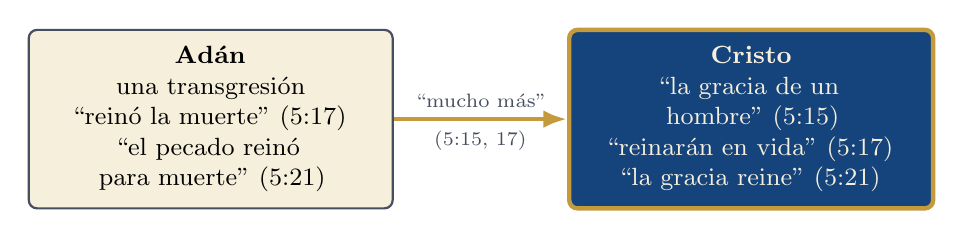
\begin{tikzpicture}[font=\small,node distance=0.8cm]
 \node[draw=gris,line width=0.8pt,fill=papiro,rounded corners=3pt,text width=4.2cm,align=center,inner sep=6pt] (a) {\textbf{Adán}\\ una transgresión\\ ``reinó la muerte'' (5:17)\\ ``el pecado reinó para muerte'' (5:21)};
 \node[draw=dorado,line width=1.6pt,fill=azul,text=papiro,rounded corners=3pt,text width=4.2cm,align=center,inner sep=6pt,right=2.2cm of a] (c) {\textbf{Cristo}\\ ``la gracia de un hombre'' (5:15)\\ ``reinarán en vida'' (5:17)\\ ``la gracia reine'' (5:21)};
 \draw[-{Latex[length=3mm]},dorado,line width=1.6pt] (a) -- node[above,font=\scriptsize,text=gris,text width=2cm,align=center] {``mucho más''} node[below,font=\scriptsize,text=gris] {(5:15, 17)} (c);
\end{tikzpicture}\par
{\footnotesize\color{gris}\textit{Figura 4.} Los dos reinos de Ro 5:12--21. \textit{Nota.} Elaboración propia.}
\end{center}

Pablo anticipa la objeción: ``¿Perseveraremos en el pecado para que la gracia abunde? En ninguna manera'' (Ro 6:1--2). Si la gracia reina, el pecado ya no es el rey: ``el pecado no se enseñoreará de vosotros; pues no estáis bajo la ley, sino bajo la gracia'' (Ro 6:14). La gracia no es permiso para pecar, sino un cambio de dueño.

\subsection{Un remanente escogido por gracia}
En Romanos 11 Pablo pregunta si Dios desechó a Israel. Responde con Elías, que creía haber quedado solo, y con la respuesta divina: ``Me he reservado siete mil hombres, que no han doblado la rodilla delante de Baal'' (1~R 19:18; Ro 11:4). Y concluye:

\begin{cita}Así también aun en este tiempo ha quedado un remanente escogido por gracia. Y si por gracia, ya no es por obras; de otra manera la gracia ya no es gracia. Y si por obras, ya no es gracia; de otra manera la obra ya no es obra.\fuente{(Ro 11:5--6)}\end{cita}

Es el texto que Pink usa como definición (sección~\ref{sec:pink-gracia}). Pablo lee la historia de Israel como la lee Deuteronomio: Israel no fue elegido por ser grande, ``sino por cuanto \SENOR{} os amó'' (Dt 7:7--8), y no recibió la tierra por su justicia: ``sabe que no es por tu justicia que \SENOR{} tu Dios te da esta buena tierra\ldots{} porque pueblo duro de cerviz eres tú'' (Dt 9:6). La gracia no es una idea que Pablo trae de fuera de Israel; es la lectura que la Torá hace de la propia historia de Israel.

\begin{nota}[Precisión]
Los debates de las últimas décadas sobre Pablo y el judaísmo (la llamada ``nueva perspectiva'') subrayan que el judaísmo del Segundo Templo no enseñaba una salvación ganada por méritos, sino una elección por gracia seguida de obediencia (Dunn, 1998; Wright, 2013). Barclay (2015) precisa que en ese judaísmo todos hablaban de gracia, pero no todos la entendían igual: Pablo acentúa que la gracia se da sin tener en cuenta el valor previo del que la recibe. Las secciones sobre el \emph{Sifré}, \emph{Avinu Malkenu} y 1QS muestran esa variedad.
\end{nota}

\subsection{``Por la gracia de Dios soy lo que soy''}
El ejemplo más claro de gracia que Pablo conoce es él mismo:

\begin{cita}Porque yo soy el más pequeño de los apóstoles, que no soy digno de ser llamado apóstol, porque perseguí a la iglesia de Dios. Pero por la gracia de Dios soy lo que soy; y su gracia no ha sido en vano para conmigo, antes he trabajado más que todos ellos; pero no yo, sino la gracia de Dios conmigo.\fuente{(1~Co 15:9--10)}\end{cita}

``Por la gracia de Dios soy lo que soy'' (\grc{χάριτι δὲ θεοῦ εἰμι ὅ εἰμι}): la frase tiene la forma de Éx 3:14 y de Éx 33:19 (\emph{idem per idem}). Lo que Pablo es, lo es por gracia; y la gracia no lo dejó pasivo: ``he trabajado más que todos ellos''. Pero corrige enseguida: ``no yo, sino la gracia de Dios conmigo''. La gracia es a la vez el don y la fuerza para responder al don.

A los gálatas les cuenta lo mismo como historia: perseguía ``sobremanera a la iglesia de Dios'' y era ``mucho más celoso de las tradiciones de mis padres'', ``pero cuando agradó a Dios, que me apartó desde el vientre de mi madre, y me llamó por su gracia'' (Gá 1:13--15). Es el Manasés del Nuevo Testamento: el peor enemigo convertido en el mayor testigo. La carta a Timoteo lo dirá como fórmula: ``Cristo Jesús vino al mundo para salvar a los pecadores, de los cuales yo soy el primero'' (1~Ti 1:15).

\begin{nota}[Precisión]
La autoría paulina de las cartas pastorales (1--2 Timoteo, Tito) se discute en la investigación. El argumento de esta sección se apoya en 1 Corintios y Gálatas, cuya autoría nadie discute; 1~Ti 1:13--16 se cita como eco de la misma experiencia.
\end{nota}

\subsection{``No desecho la gracia de Dios''}
En Gálatas, Pablo enfrenta a quienes exigían a los gentiles la circuncisión para pertenecer al pueblo de Dios. Su conclusión usa otra vez el adverbio \grc{δωρεάν}:

\begin{cita}No desecho la gracia de Dios; pues si por la ley fuese la justicia, entonces por demás murió Cristo.\fuente{(Gá 2:21)}\end{cita}

``Por demás'' traduce \grc{δωρεάν}: ``de balde'', ``en vano''. Si la justicia se pudiera ganar, la muerte de Cristo habría sido \emph{jinnam} en el peor sentido: inútil. Pablo usa la misma palabra para lo que Dios da gratis (Ro 3:24) y para lo que sería la cruz si las obras bastaran (Gá 2:21). La gracia se rechaza no solo pecando, sino también intentando pagarla.

\subsection{Efesios: de muertos a hechura suya}
La carta a los Efesios resume la gracia en un párrafo que recorre todo el arco de Gn 6 a Romanos 5:

\begin{cita}Pero Dios, que es rico en misericordia, por su gran amor con que nos amó, aun estando nosotros muertos en pecados, nos dio vida juntamente con Cristo (por gracia sois salvos)\ldots{} Porque por gracia sois salvos por medio de la fe; y esto no de vosotros, pues es don de Dios; no por obras, para que nadie se gloríe. Porque somos hechura suya, creados en Cristo Jesús para buenas obras, las cuales Dios preparó de antemano para que anduviésemos en ellas.\fuente{(Ef 2:4--5, 8--10)}\end{cita}

\begin{filologia}[Ef 2:8--10]
\begin{tabular}{@{}L{3.6cm}L{1.6cm}L{9.6cm}@{}}
\grc{τῇ γὰρ χάριτί ἐστε σεσῳσμένοι} & \grc{σῴζω} & ``por la gracia estáis salvados'': participio perfecto, una salvación cumplida que permanece. \\[2pt]
\grc{θεοῦ τὸ δῶρον} & \grc{δῶρον} & ``de Dios es el don'': el don es todo el conjunto (salvación por gracia mediante la fe). \\[2pt]
\grc{ποίημα} \emph{poíēma} & \grc{ποιέω} & ``hechura'', ``obra hecha'': Dios es el artesano. \\[2pt]
\grc{ἐπὶ ἔργοις ἀγαθοῖς} & \grc{ἔργον} & ``para buenas obras'': las obras no son la causa de la gracia, sino su propósito. \\
\end{tabular}
\end{filologia}

El texto cierra la objeción que Pink temía y la que temía Pablo. La gracia excluye las obras como causa (``no por obras'') y las produce como fruto (``para buenas obras''). Ef 1:6 añade el fin último: todo es ``para alabanza de la gloria de su gracia, con la cual nos hizo aceptos (\grc{ἐχαρίτωσεν}) en el Amado''. El verbo, de la raíz de \grc{χάρις}, significa ``agraciar'': Dios hace agraciados a los que no tenían gracia.

\begin{nota}[Precisión]
La autoría paulina de Efesios se discute. Su doctrina de la gracia coincide con la de Romanos y Gálatas (Ro 3:24; 4:4--5; 11:6; Gá 2:16, 21), cartas cuya autoría no se discute.
\end{nota}

\subsection{``Gracia y paz''}\label{sec:gracia-paz}
Casi todas las cartas de Pablo comienzan con el mismo saludo: \grc{χάρις ὑμῖν καὶ εἰρήνη ἀπὸ θεοῦ πατρὸς ἡμῶν καὶ κυρίου Ἰησοῦ Χριστοῦ}, ``Gracia y paz a vosotros, de Dios nuestro Padre y del Señor Jesucristo'' (Ro 1:7; 1~Co 1:3; 2~Co 1:2; Gá 1:3; Flp 1:2) y terminan con ``la gracia de nuestro Señor Jesucristo sea con vosotros'' (Ro 16:20; Gá 6:18). La gracia abre y cierra cada carta.

El saludo griego habitual era \grc{χαίρειν} (``alégrate'', Hch 15:23; Stg 1:1); el saludo judío, \emph{shalom}. Pablo cambia \grc{χαίρειν} por \grc{χάρις}, una palabra de sonido parecido, y le añade la paz. La bendición sacerdotal había terminado igual: ``y te dé gracia\ldots{} y ponga en ti paz'' (Nm 6:25--26).

\begin{nota}[Precisión]
Que el saludo paulino ``gracia y paz'' sea un eco de la bendición de Nm 6:24--26 es una lectura posible que algunos intérpretes proponen; Pablo no cita el texto, y la Septuaginta traduce \emph{viyjunnekka} con \grc{ἐλεήσαι σε}, no con \grc{χάρις}. Lo seguro es que la fórmula une un término griego transformado (\grc{χάρις} en lugar de \grc{χαίρειν}) con el \emph{shalom} hebreo.
\end{nota}

\subsection{La gracia de Cristo, que se hizo pobre}
Pablo no habla de la gracia como una fuerza impersonal. La gracia tiene rostro:

\begin{cita}Porque ya conocéis la gracia de nuestro Señor Jesucristo, que por amor a vosotros se hizo pobre, siendo rico, para que vosotros con su pobreza fueseis enriquecidos.\fuente{(2~Co 8:9)}\end{cita}

La gracia de Cristo es un intercambio: su riqueza por nuestra pobreza. Es la misma estructura que Pablo describe en la cruz: ``Al que no conoció pecado, por nosotros lo hizo pecado, para que nosotros fuésemos hechos justicia de Dios en él'' (2~Co 5:21). Juan la dice con el vocabulario del Sinaí: el Verbo ``habitó entre nosotros (y vimos su gloria\ldots), lleno de gracia y de verdad\ldots{} Porque de su plenitud tomamos todos, y gracia sobre gracia. Pues la ley por medio de Moisés fue dada, pero la gracia y la verdad vinieron por medio de Jesucristo'' (Jn 1:14, 16--17).

\begin{center}\small\renewcommand{\arraystretch}{1.22}
\begin{tabular}{@{}L{2.6cm}L{4.6cm}L{3.6cm}L{3.6cm}@{}}
\toprule
\textbf{Texto} & \textbf{Hebreo (TM)} & \textbf{Septuaginta} & \textbf{Juan} \\ \midrule
Éx 34:6 & \heb{וְרַב־חֶסֶד וֶאֱמֶת} & \grc{πολυέλεος καὶ ἀληθινός} & --- \\
Jn 1:14 & --- & --- & \grc{πλήρης χάριτος καὶ ἀληθείας} \\
Éx 33:18 / Jn 1:14 & \heb{הַרְאֵנִי נָא אֶת־כְּבֹדֶךָ} & \grc{δεῖξόν μοι τὴν σεαυτοῦ δόξαν} & \grc{ἐθεασάμεθα τὴν δόξαν αὐτοῦ} \\
\bottomrule
\end{tabular}\par
{\footnotesize\color{gris}\textit{Tabla 6.} Éxodo 33--34 y Juan 1. \textit{Nota.} Elaboración propia con la BHS, la LXX y NA28.}
\end{center}

Moisés pidió ver la gloria y Dios proclamó su Nombre ``grande en \emph{jésed} y \emph{emet}''. Juan dice que en el Verbo hecho carne se vio esa gloria, ``llena de gracia y de verdad''. Donde la Septuaginta había traducido \emph{jésed} con \grc{ἔλεος}, Juan usa \grc{χάρις}: en Cristo, el amor leal del pacto se muestra como gracia.

\begin{nota}[Precisión]
El eco de Éx 34:6 en Jn 1:14 es ampliamente reconocido por los comentaristas (véase la introducción de esta obra), pero Juan no cita el texto. Juan no es Pablo; se incluye aquí porque Pink basa en Jn 1:17 su afirmación de que la gracia fue ``completamente revelada'' en Cristo.
\end{nota}

\subsection{``Bástate mi gracia''}
La gracia no solo salva: sostiene. Pablo pidió tres veces que le fuera quitado ``un aguijón en mi carne''. La respuesta fue otra:

\begin{cita}Y me ha dicho: Bástate mi gracia; porque mi poder se perfecciona en la debilidad. Por tanto, de buena gana me gloriaré más bien en mis debilidades, para que repose sobre mí el poder de Cristo.\fuente{(2~Co 12:9)}\end{cita}

\grc{Ἀρκεῖ σοι ἡ χάρις μου}: ``te basta mi gracia''. El verbo \grc{ἀρκέω} es ``ser suficiente''. La gracia que justifica al impío es la misma que sostiene al débil. Y otra vez aparece Jer 9:24: Pablo solo se gloría en lo que muestra el poder de Dios, no el suyo.

\subsection{La gracia que enseña}
La carta a Tito une la gracia con la vida diaria:

\begin{cita}Porque la gracia de Dios se ha manifestado para salvación a todos los hombres, enseñándonos que, renunciando a la impiedad y a los deseos mundanos, vivamos en este siglo sobria, justa y piadosamente, aguardando la esperanza bienaventurada y la manifestación gloriosa de nuestro gran Dios y Salvador Jesucristo.\fuente{(Tit 2:11--13)}\end{cita}

La gracia ``se manifestó'' (\grc{ἐπεφάνη}), como una luz que aparece, y ``enseña'' (\grc{παιδεύουσα}), como un maestro que educa. La gracia que perdona también forma. Es la respuesta definitiva a Ro 6:1: quien ha recibido la gracia no busca una excusa para pecar, sino que aprende de ella a vivir.

%===================================================================
\section{Aplicación: un atributo comunicable}

\subsection{``De gracia recibisteis, dad de gracia''}
La gracia, en su fuente, es solo de Dios: solo él justifica al impío. Pero el que la recibe la refleja. Jesús lo mandó al enviar a los doce: ``de gracia recibisteis, dad de gracia'' (\grc{δωρεὰν ἐλάβετε, δωρεὰν δότε}, Mt 10:8). Pablo predicó el evangelio ``de balde'' (\grc{δωρεάν}, 2~Co 11:7), y llamó ``gracia'' a la ofrenda de las iglesias de Macedonia para los pobres de Jerusalén: ``os hacemos saber la gracia de Dios que se ha dado a las iglesias de Macedonia\ldots{} abundad también en esta gracia'' (2~Co 8:1, 7). La generosidad del creyente es la gracia de Dios que sigue circulando.

\subsection{La gracia en la palabra y en el perdón}
El Nuevo Testamento aplica la gracia a dos terrenos concretos. El primero es la palabra: ``Sea vuestra palabra siempre con gracia, sazonada con sal'' (Col 4:6); que salga de la boca la palabra ``buena para la necesaria edificación, a fin de dar gracia a los oyentes'' (Ef 4:29). El segundo es el perdón: ``sed benignos unos con otros, misericordiosos, perdonándoos unos a otros, como Dios también os perdonó a vosotros en Cristo'' (Ef 4:32). ``Perdonar'' es aquí \grc{χαρίζομαι}: dar gracia. El que perdona da al otro lo que no merece, como lo recibió.

\subsection{Cinco respuestas}
\begin{enumerate}
\item \textbf{Recibir con las manos vacías.} La gracia se recibe como la recibió Manasés, con una \emph{tejinná}, o como la pide la sinagoga: ``ten gracia de nosotros\ldots{} porque no hay en nosotros obras''. Quien trae algo para pagar todavía no ha entendido el regalo (Ro 4:4--5; Is 55:1).
\item \textbf{No convertir la gracia en permiso.} ``¿Perseveraremos en el pecado para que la gracia abunde? En ninguna manera'' (Ro 6:1--2). La gracia que perdona también enseña a renunciar a la impiedad (Tit 2:11--12).
\item \textbf{Vivir en gratitud y humildad.} ``¿Qué tienes que no hayas recibido?'' (1~Co 4:7). Dios ``da gracia a los humildes'' (Pr 3:34; Stg 4:6): la humildad es la forma de la mano que la recibe. En griego, gracia y gracias son la misma palabra.
\item \textbf{Dar y perdonar de gracia.} ``De gracia recibisteis, dad de gracia'' (Mt 10:8). La medida no es lo que el otro merece, sino lo que uno recibió (Ef 4:32; Lc 6:32--35).
\item \textbf{Acercarse al trono de la gracia.} ``Acerquémonos, pues, confiadamente al trono de la gracia, para alcanzar misericordia y hallar gracia para el oportuno socorro'' (He 4:16). La fórmula de Noé (``halló gracia'') se vuelve invitación: el trono del juez es, en Cristo, el lugar donde se halla gracia.
\end{enumerate}

%===================================================================
\section{Síntesis}

\begin{tcolorbox}[colback=papiro,colframe=azul,boxrule=1pt,arc=3pt,fonttitle=\bfseries,title=La gracia de Dios]
La gracia es el favor inmerecido de Dios hacia pecadores. La halló Noé cuando toda carne estaba bajo sentencia (Gn 6:8); la proclamó Dios en su Nombre ante un pueblo infiel, ``misericordioso y clemente'' (Éx 34:6); la cantó David en su pecado (Sal 51:1) y la recibió Manasés en sus cadenas (2~Cr 33:13). Es gratuita como el esclavo que sale libre ``de balde'' (Éx 21:2; Is 52:3), soberana (Éx 33:19), eterna (2~Ti 1:9) y abundante, porque ``cuando el pecado abundó, sobreabundó la gracia'' (Ro 5:20). Su plenitud está en Cristo, ``lleno de gracia y de verdad'' (Jn 1:14), en quien somos ``justificados gratuitamente por su gracia'' (Ro 3:24) para alabanza de su gloria (Ef 1:6).
\end{tcolorbox}

\begin{center}\small\renewcommand{\arraystretch}{1.22}
\begin{tabular}{@{}L{3.2cm}L{6.8cm}L{4.4cm}@{}}
\toprule
\textbf{Lente} & \textbf{Aporte al atributo} & \textbf{Textos} \\ \midrule
Texto ancla & la gracia aparece en el peor momento de la humanidad & Gn 6:5--8; 8:21 \\
La palabra & \emph{jen}: el favor que se halla en los ojos del superior; \emph{jinnam}: de balde & Rt 2:10; Éx 21:2; Is 52:3 \\
El Nombre & \emph{jannun}: el que oye al que no puede reclamar & Éx 22:27; 34:6; Jon 4:2 \\
Pink & la gracia excluye el mérito; es eterna, gratuita y soberana & Ro 11:6; 2~Ti 1:9; Ro 5:21 \\
Israel & Manasés oído en su súplica & 2~Cr 33:12--13 \\
Judaísmo & ``don gratuito''; ``aunque no lo merezca''; ``no hay en nosotros obras'' & Dt 3:23; Éx 33:19; \emph{Avinu Malkenu} \\
Pablo & justificados gratuitamente; la gracia sobreabunda y reina; ``soy lo que soy'' & Ro 3:24; 5:20--21; 1~Co 15:10 \\
Vida & dar de gracia, perdonar, hablar con gracia & Mt 10:8; Ef 4:32; Col 4:6 \\
\bottomrule
\end{tabular}\end{center}

Así, la gracia une el principio y el fin de esta obra. La gloria de Dios es la comunión de sus perfecciones, y esa plenitud habita en Cristo (Col 2:9). La gracia es la perfección por la cual esa gloria, que el pecador había perdido (Ro 3:23), le es dada otra vez: ``gracia y gloria dará \SENOR'' (Sal 84:11).

%===================================================================
\section*{Glosario}\markboth{Glosario}{}
\begin{description}
\item[\emph{Avinu Malkenu}] (\heb{אָבִינוּ מַלְכֵּנוּ}). ``Padre nuestro, Rey nuestro'': oración judía de los días penitenciales; incluye ``ten gracia de nosotros\ldots{} porque no hay en nosotros obras''.
\item[\emph{Dōreán}] (\grc{δωρεάν}). ``Gratuitamente'', ``de balde'', ``sin causa'': traducción griega de \emph{jinnam} (Ro 3:24; Gá 2:21; Jn 15:25).
\item[\emph{Jannun}] (\heb{חַנּוּן}). ``Clemente'': adjetivo que en la Biblia hebrea se dice casi solo de Dios (Éx 22:27; 34:6).
\item[\emph{Janán}] (\heb{חָנַן}). ``Mostrar gracia'', ``favorecer''; en hitpael, ``suplicar gracia'' (Dt 3:23).
\item[\emph{Járis}] (\grc{χάρις}). ``Gracia'', ``favor'', ``agradecimiento'': palabra central de Pablo (Ro 3:24; Ef 2:8).
\item[\emph{Járisma}] (\grc{χάρισμα}). ``Don'', ``dádiva'': el regalo concreto de la gracia (Ro 6:23).
\item[\emph{Jen}] (\heb{חֵן}). ``Gracia'', ``favor'', ``encanto'': lo que se halla ``en los ojos'' de otro (Gn 6:8).
\item[\emph{Jinnam}] (\heb{חִנָּם}). ``De balde'', ``gratis'', ``sin causa'': adverbio formado de \emph{jen} (Éx 21:2; Is 52:3).
\item[\emph{Matnat jinnam}] (\heb{מַתְּנַת חִנָּם}). ``Don gratuito'': expresión de Rashi y del \emph{Sifré} para lo que piden los justos en la oración.
\item[\emph{Opsōnia}] (\grc{ὀψώνια}). ``Paga'', ``salario'' del soldado: lo que el pecado paga (Ro 6:23).
\item[\emph{Tejinná}] (\heb{תְּחִנָּה}). ``Súplica'', ``pedido de gracia'' (2~Cr 33:13; 1~R 8:28).
\end{description}

%===================================================================
\section*{Referencias}\markboth{Referencias}{}
\refapa{Barclay, J.~M.~G. (2015). \emph{Paul and the gift}. Eerdmans.}
\refapa{Bauer, W., Danker, F.~W., Arndt, W.~F., \& Gingrich, F.~W. (2000). \emph{A Greek-English lexicon of the New Testament and other early Christian literature} (3.ª ed.). University of Chicago Press.}
\refapa{\emph{Bereshit Rabá} [29:1, 3]. (s.f.). Sefaria. \url{https://www.sefaria.org}}
\refapa{Berkhof, L. (1938). \emph{Systematic theology}. Eerdmans.}
\refapa{Brown, F., Driver, S.~R., \& Briggs, C.~A. (1906). \emph{A Hebrew and English lexicon of the Old Testament}. Clarendon Press.}
\refapa{Cassuto, U. (1961). \emph{A commentary on the book of Genesis: Part I. From Adam to Noah} (I. Abrahams, Trad.). Magnes Press.}
\refapa{Dunn, J.~D.~G. (1988). \emph{Romans 1--8} (Word Biblical Commentary 38A). Word Books.}
\refapa{Dunn, J.~D.~G. (1998). \emph{The theology of Paul the apostle}. Eerdmans.}
\refapa{Elbogen, I. (1993). \emph{Jewish liturgy: A comprehensive history} (R.~P. Scheindlin, Trad.). Jewish Publication Society.}
\refapa{Elliger, K., \& Rudolph, W. (Eds.). (1997). \emph{Biblia Hebraica Stuttgartensia} (5.ª ed.). Deutsche Bibelgesellschaft.}
\refapa{Guggenheimer, H.~W. (Ed. y Trad.). (1999--2015). \emph{The Jerusalem Talmud} [Sanedrín 10:2]. De Gruyter. Sefaria. \url{https://www.sefaria.org}}
\refapa{Koehler, L., \& Baumgartner, W. (2001). \emph{The Hebrew and Aramaic lexicon of the Old Testament} (M.~E.~J. Richardson, Trad.; Ed. de estudio). Brill.}
\refapa{Moo, D.~J. (1996). \emph{The epistle to the Romans}. Eerdmans.}
\refapa{Nestle, E., \& Aland, K. (Eds.). (2012). \emph{Novum Testamentum Graece} (28.ª ed.). Deutsche Bibelgesellschaft.}
\refapa{Pink, A. W. (2020). \emph{Los atributos de Dios} (E. Rodríguez Cruz, Trad.). Chapel Library. (Obra original publicada en 1930)}
\refapa{Rahlfs, A., \& Hanhart, R. (Eds.). (2006). \emph{Septuaginta} (Ed. rev.). Deutsche Bibelgesellschaft.}
\refapa{Rashi. (s.f.). \emph{Comentario a la Torá} [Dt 3:23]. Sefaria. \url{https://www.sefaria.org}}
\refapa{\emph{Santa Biblia: Reina-Valera 1960}. (1960). Sociedades Bíblicas en América Latina.}
\refapa{Sasson, J.~M. (1975). Word-play in Gen 6:8--9. \emph{The Catholic Biblical Quarterly, 37}(2), 165--166.}
\refapa{\emph{Shemot Rabá} [3:6]. (s.f.). Sefaria. \url{https://www.sefaria.org}}
\refapa{\emph{Sidur Ashkenaz} [Amidá; Birkat hamazón] y \emph{Sidur Sefard} [Avinu Malkenu]. (s.f.). Sefaria. \url{https://www.sefaria.org}}
\refapa{\emph{Sifré Devarim} [26]. (s.f.). Sefaria. \url{https://www.sefaria.org}}
\refapa{Steinsaltz, A. (Ed.). (2017). \emph{Koren Talmud Bavli: Edición William Davidson} [Berajot 7a; Taanit 25b; Sanedrín 103a; 108a]. Sefaria. \url{https://www.sefaria.org}}
\refapa{\emph{The Mishnah} [Sanedrín 10:2]. (s.f.). Sefaria. \url{https://www.sefaria.org}}
\refapa{Vermes, G. (2004). \emph{The complete Dead Sea Scrolls in English} (Ed. rev.). Penguin.}
\refapa{Wright, N.~T. (2013). \emph{Paul and the faithfulness of God}. Fortress Press.}
\end{document}
